% !TEX root = ../main.tex

% ==========================================================================
% ANEXO A: ANILLO DENSO
%==========================================================================
\section{Ajustes Armónicos para el Anillo Denso}
\label{anexo:ajustes_anillo_denso}

En esta sección se presenta la inspección visual del ajuste armónico realizado sobre la señal total del Detector de Superficie (SD) en el entorno del Anillo Denso. Como fue discutido en la Sección \ref{subsec:mc_vs_rec}, los elevados valores de $\chi^2/\text{ndf}$ obtenidos para el SD no responden a una falla fenomenológica del modelo dipolar, sino a la extrema reducción de la incertidumbre estadística (consecuencia de la alta afluencia de partículas electromagnéticas) que vuelve al ajuste hipersensible a fluctuaciones de segundo orden. 

En la Figura \ref{fig:anexo_ajuste_sd_bin9} se expone el ajuste representativo para el bin radial correspondiente a $r = 450$~m, evidenciando que la curva armónica captura con precisión la tendencia macroscópica de la asimetría a pesar del castigo estadístico de los residuos.

\begin{figure}[H]
	\centering
	% Ajustá la extensión (.pdf o .png) según corresponda
	
\includegraphics[width=0.95\textwidth]{capitulos/imagenes_capitulos/anexo/Ajuste_SD_Total_Bin9.pdf}
	\caption{Ajuste armónico de la señal total del SD en el Anillo Denso para el bin radial centrado en $450$~m. Las barras de error (error estándar de la media) resultan imperceptibles debido a la masiva estadística electromagnética. Se observa que el modelo de primer orden describe correctamente la tendencia general de la asimetría azimutal.}
	\label{fig:anexo_ajuste_sd_bin9}
\end{figure}


% ==========================================================================
% ANEXO B: INFILL
%==========================================================================
\section{Grillas de Ajustes Armónicos para el Arreglo \textit{Infill} en simulaciones}
\label{anexo:ajustes_infill}

En este anexo se presentan las grillas completas de los ajustes armónicos realizados sobre las simulaciones del arreglo \textit{Infill} tanto usando la geometria verdadera como la reconstruida. Cada figura corresponde a un rango cenital específico ($\Delta\theta = 10^\circ$) y expone la evolución de los cinco observables físicos analizados a lo largo de los sucesivos bines radiales ($\Delta r = 150$~m). 

Para cada celda del espacio de fases, se reportan los datos experimentales simulados, el ajuste al armónico de primer orden superpuesto, y los estadísticos de bondad de ajuste correspondientes ($A_1$ y $\chi^2/\text{ndf}$).

\newpage

% Iniciamos el modo apaisado para las figuras anchas
\begin{landscape}
	
	% --- Geometría Monte Carlo ---
	\subsection{Geometría Verdadera (Monte Carlo)}
	\label{anexo:ajustes_infill_mc}
	
	% --- Bin 0 - 10 ---
	\begin{figure}[H]
		\centering
		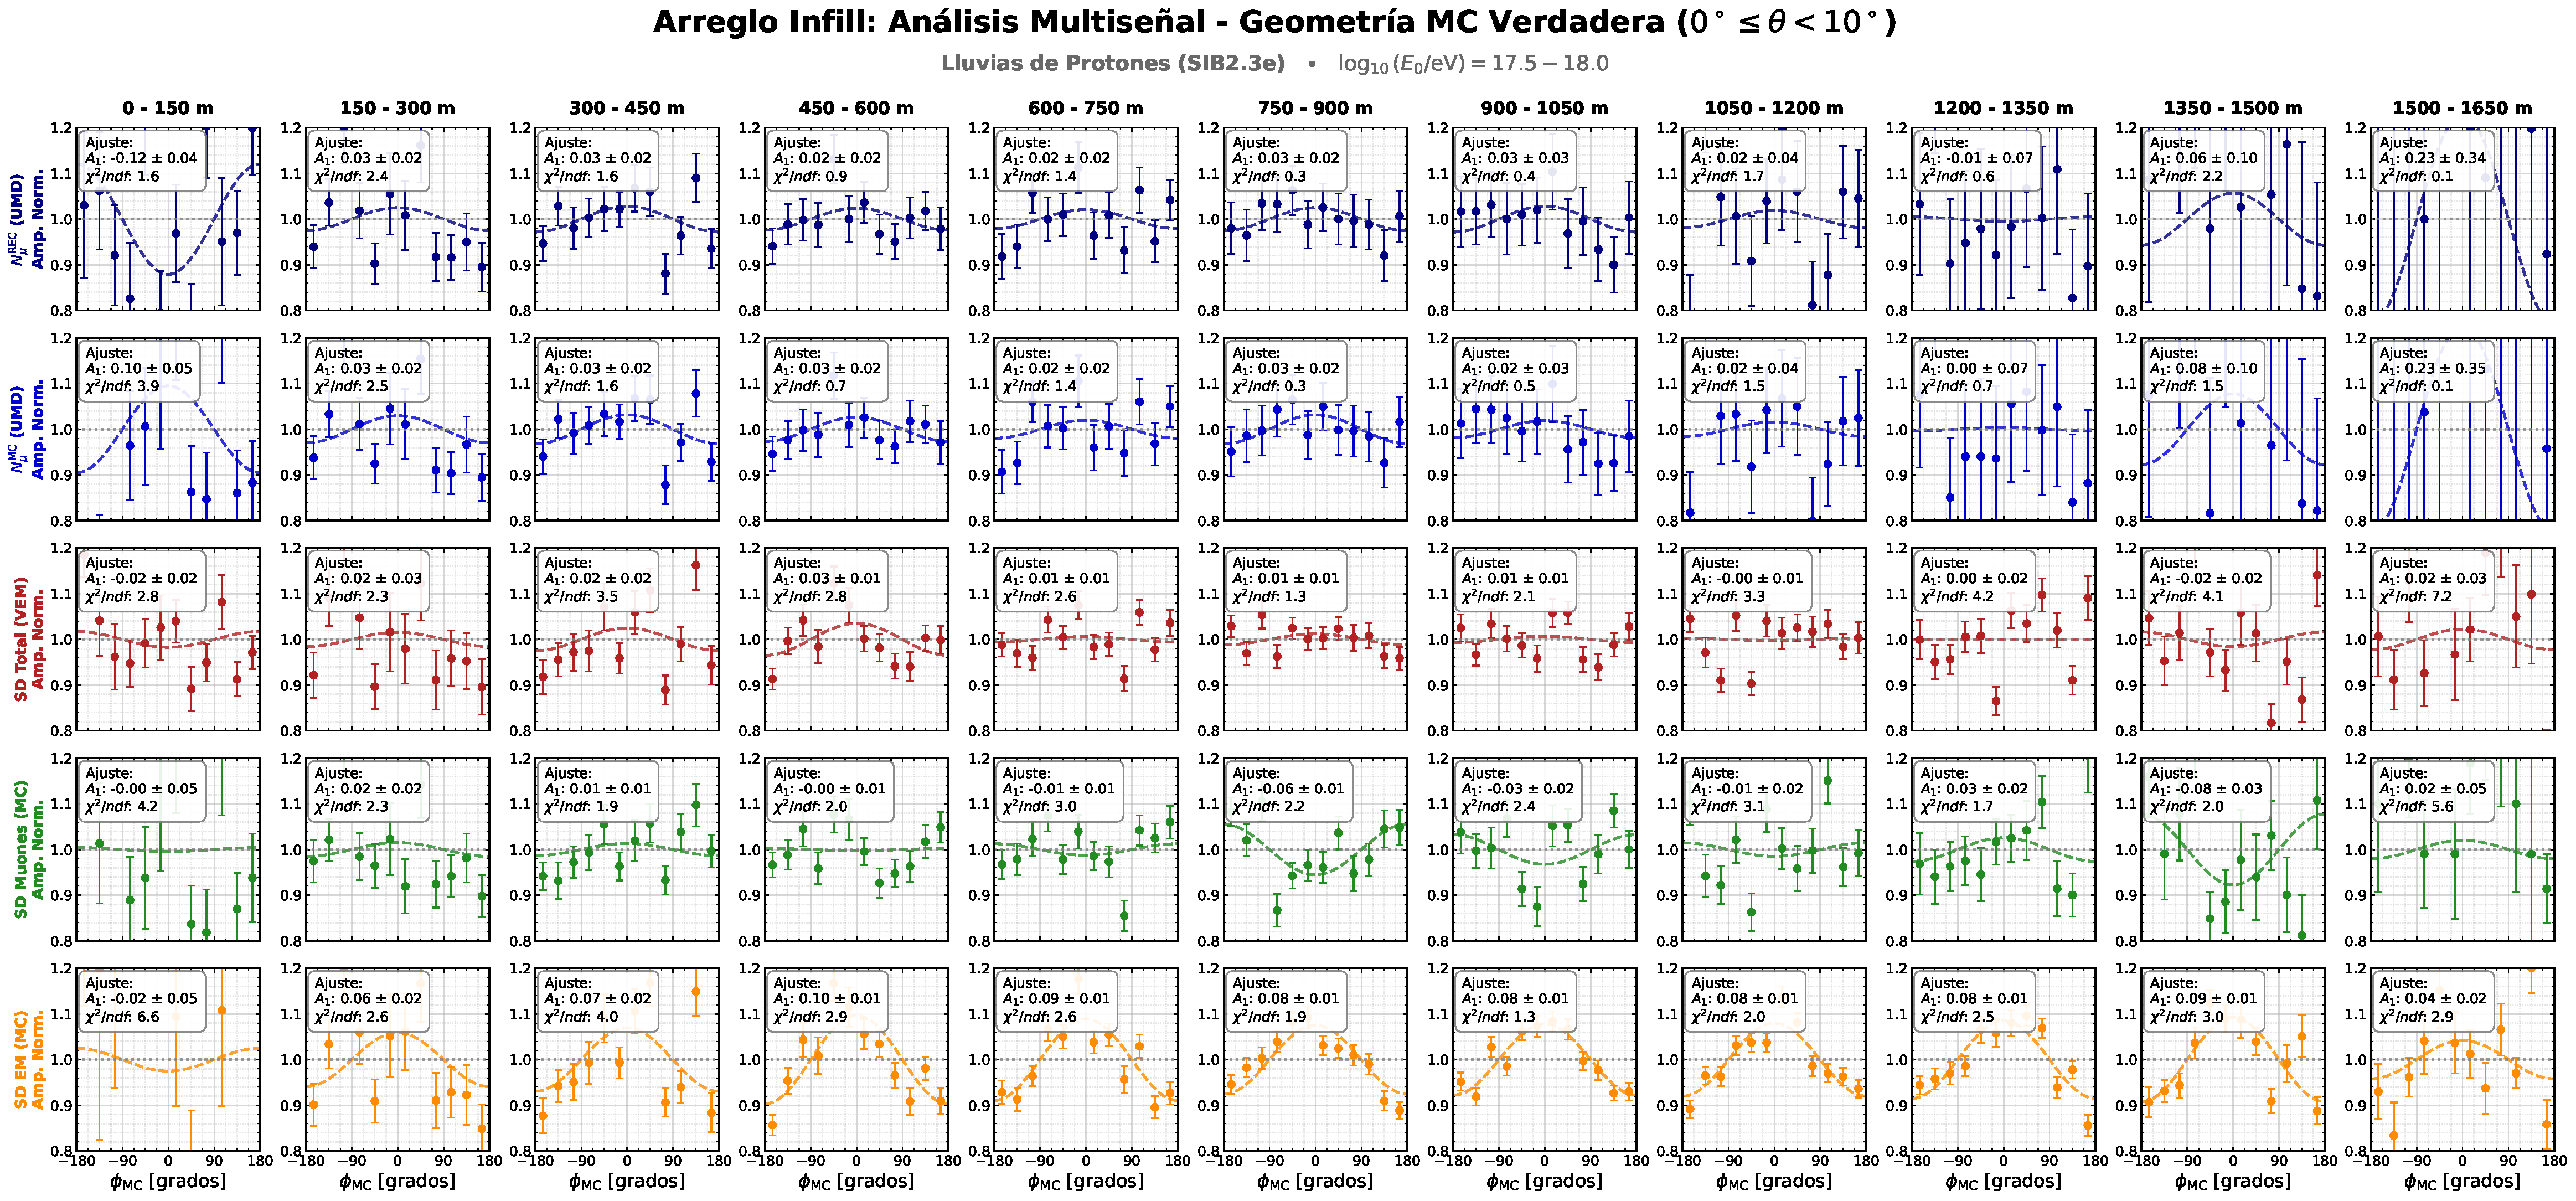
\includegraphics[width=1\linewidth]{capitulos/imagenes_capitulos/anexo/Anexo_Grilla_MC_0_10.pdf}
		\caption{Análisis multiseñal de asimetría azimutal forzando la geometría Monte Carlo para lluvias con ángulos cenitales verdaderos entre $0^\circ$ y $10^\circ$. Las barras de error representan el error estándar de la media en cada bin angular.}
		\label{fig:anexo_grilla_mc_0_10}
	\end{figure}
	\clearpage
	
	% --- Bin 10 - 20 ---
	\begin{figure}[H]
		\centering
		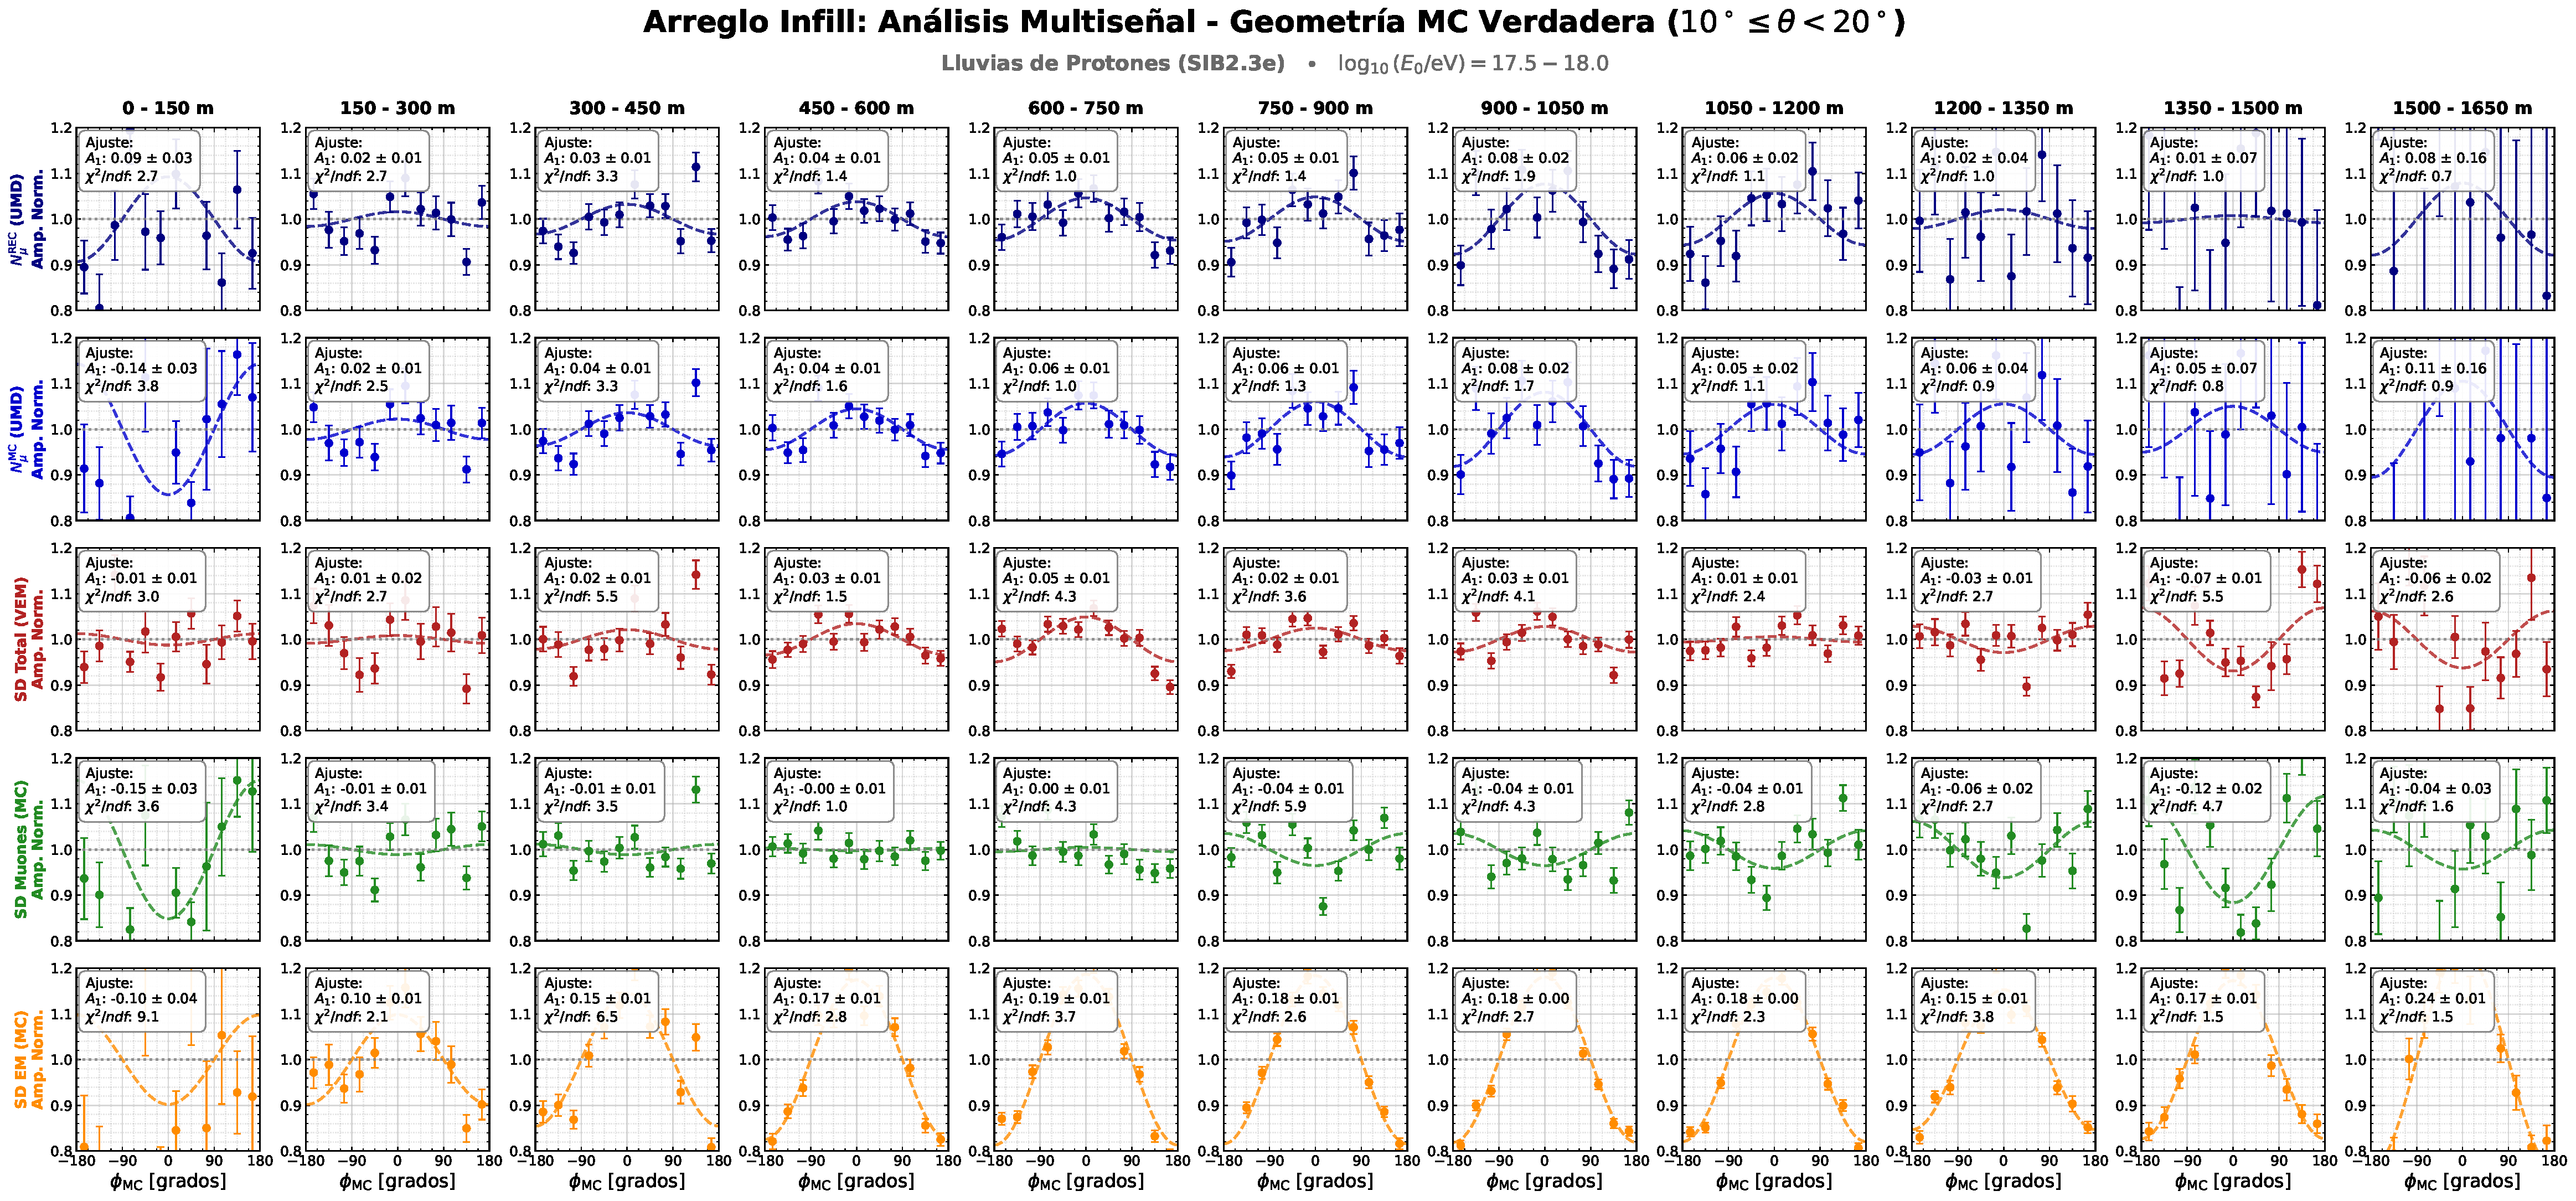
\includegraphics[width=\linewidth]{capitulos/imagenes_capitulos/anexo/Anexo_Grilla_MC_10_20.pdf}
		\caption{Análisis multiseñal de asimetría azimutal forzando la geometría Monte Carlo para lluvias con ángulos cenitales verdaderos entre $10^\circ$ y $20^\circ$.}
		\label{fig:anexo_grilla_mc_10_20}
	\end{figure}
	\clearpage
	
	% --- Bin 20 - 30 ---
	\begin{figure}[H]
		\centering
		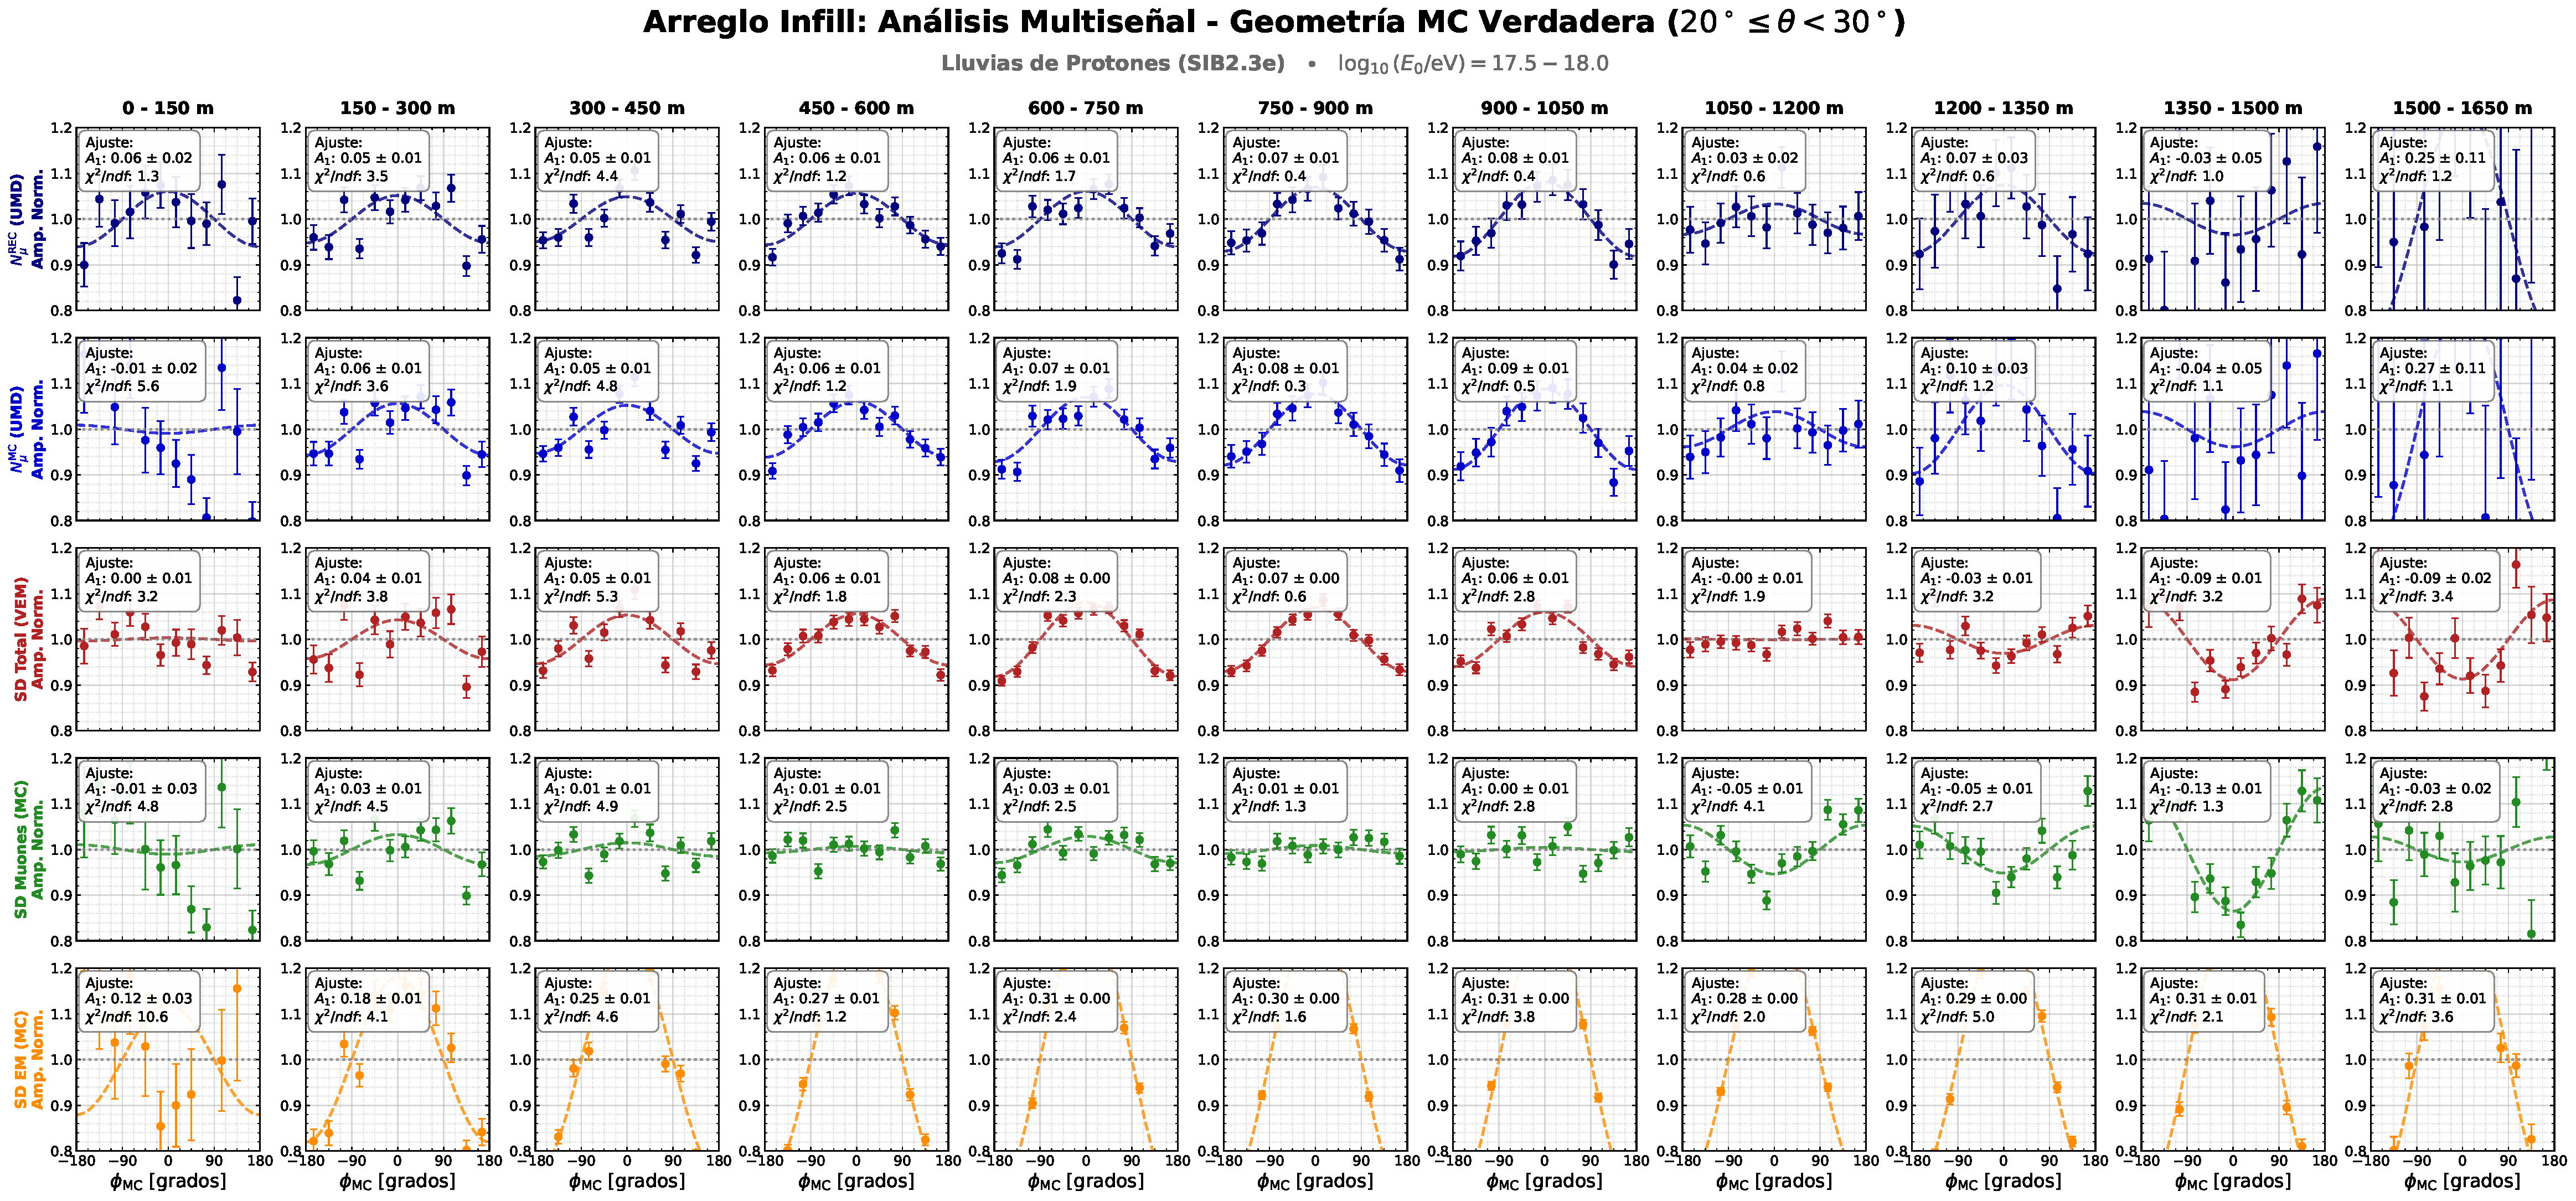
\includegraphics[width=\linewidth]{capitulos/imagenes_capitulos/anexo/Anexo_Grilla_MC_20_30.pdf}
		\caption{Análisis multiseñal de asimetría azimutal forzando la geometría Monte Carlo para lluvias con ángulos cenitales verdaderos entre $20^\circ$ y $30^\circ$.}
		\label{fig:anexo_grilla_mc_20_30}
	\end{figure}
	\clearpage
	
	% --- Bin 30 - 40 ---
	\begin{figure}[H]
		\centering
		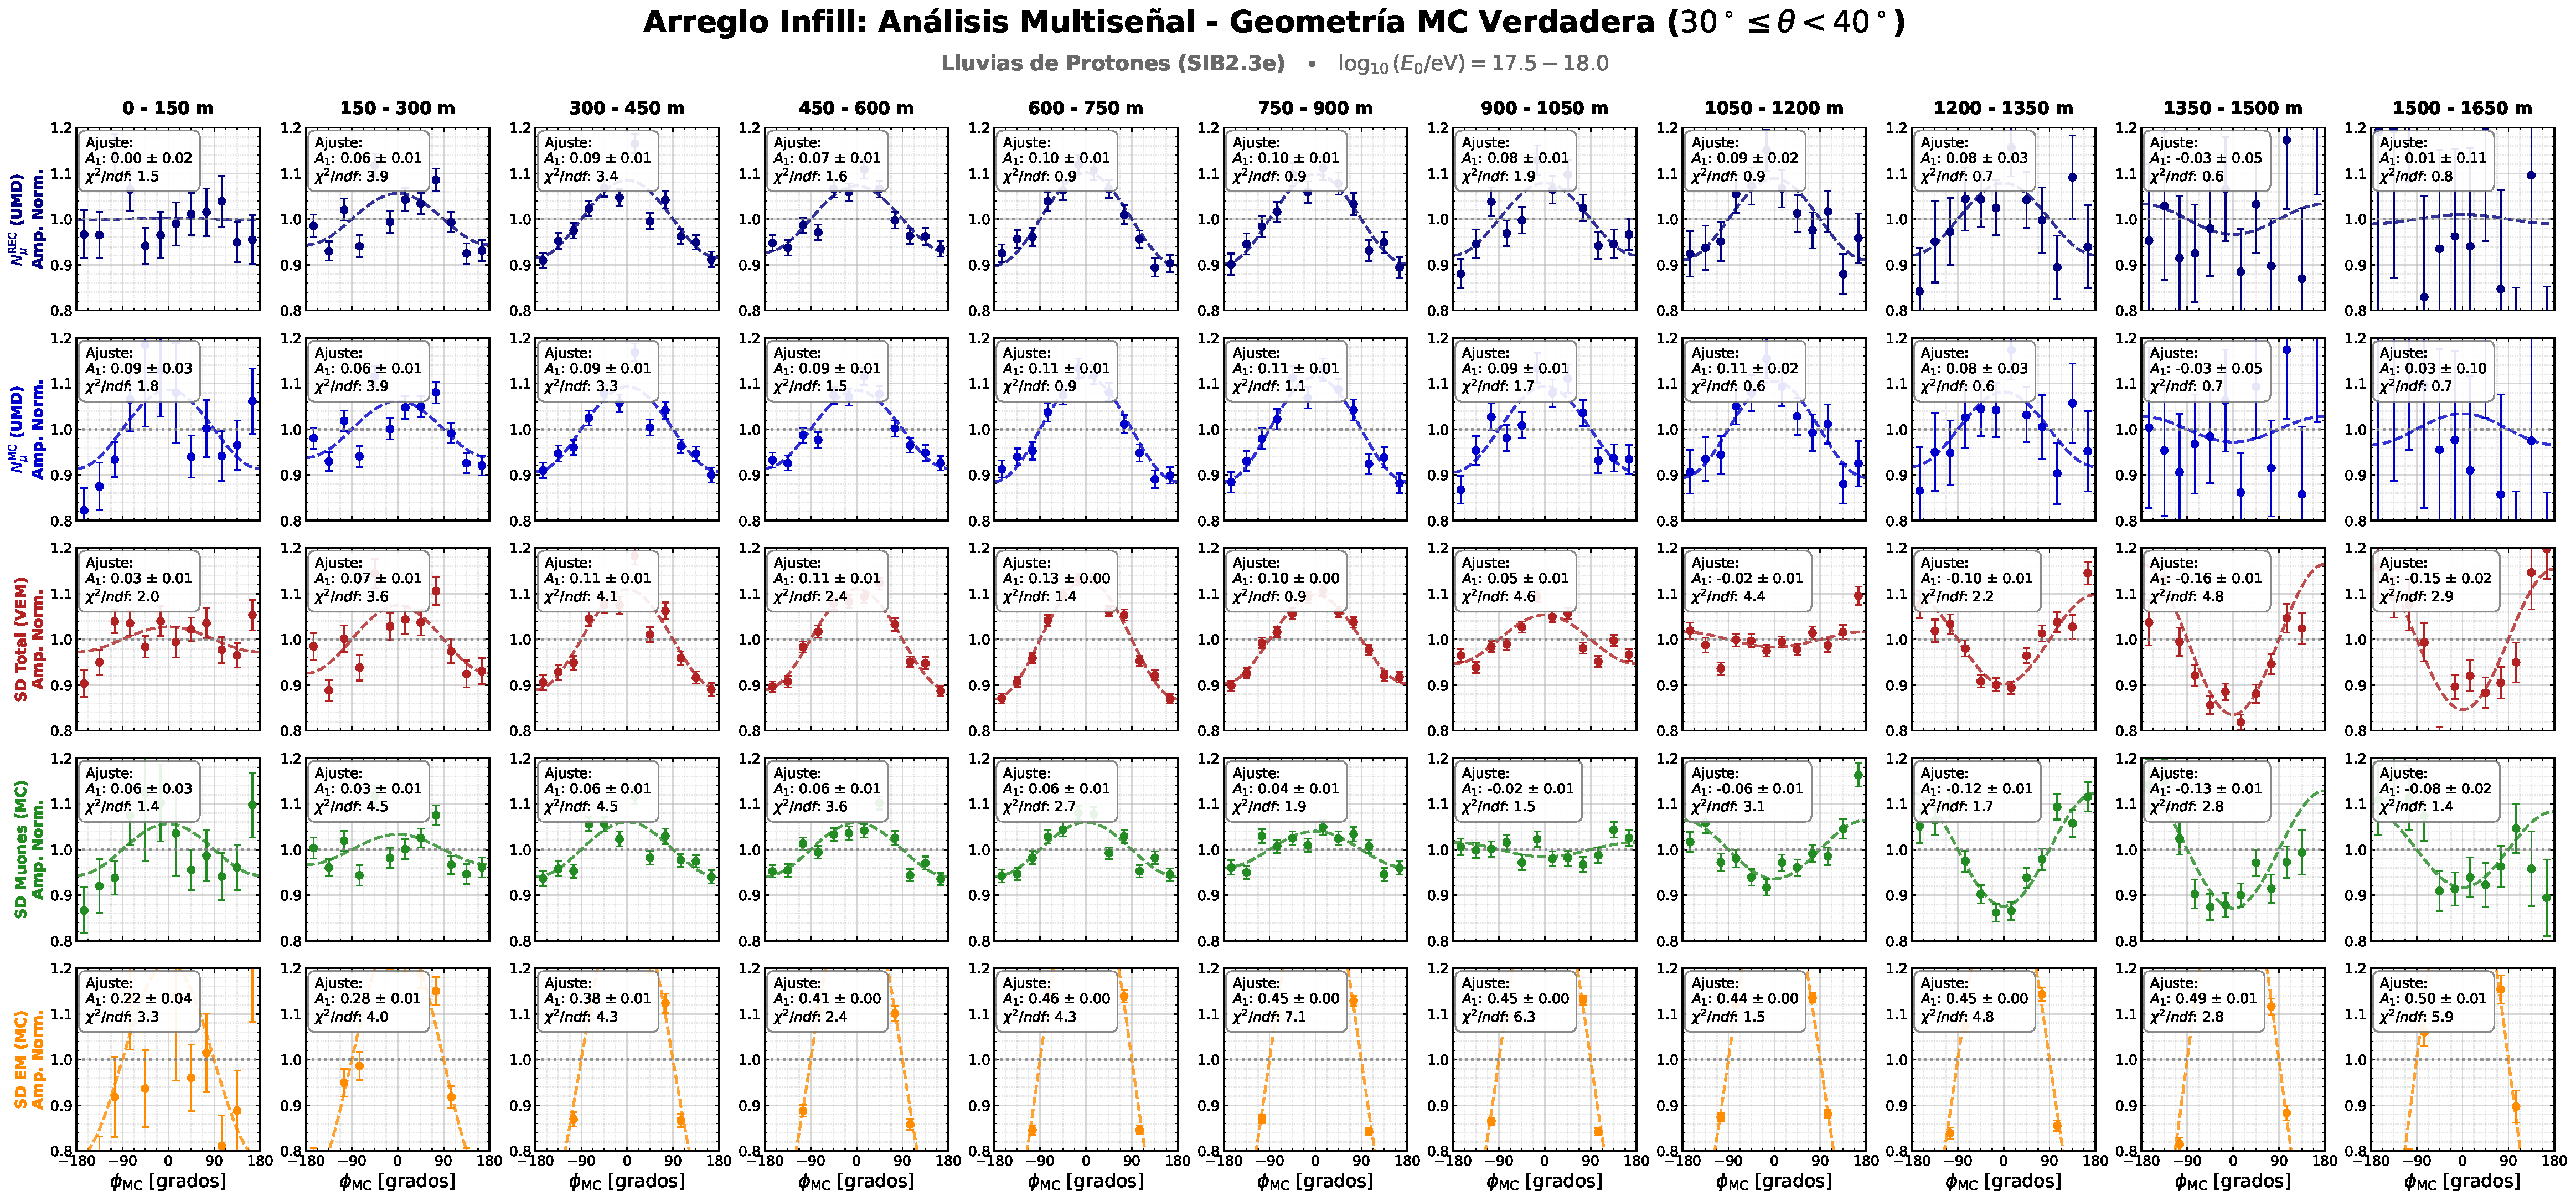
\includegraphics[width=\linewidth]{capitulos/imagenes_capitulos/anexo/Anexo_Grilla_MC_30_40.pdf}
		\caption{Análisis multiseñal de asimetría azimutal forzando la geometría Monte Carlo para lluvias con ángulos cenitales verdaderos entre $30^\circ$ y $40^\circ$.}
		\label{fig:anexo_grilla_mc_30_40}
	\end{figure}
	\clearpage
	
	% --- Bin 40 - 50 ---
	\begin{figure}[H]
		\centering
		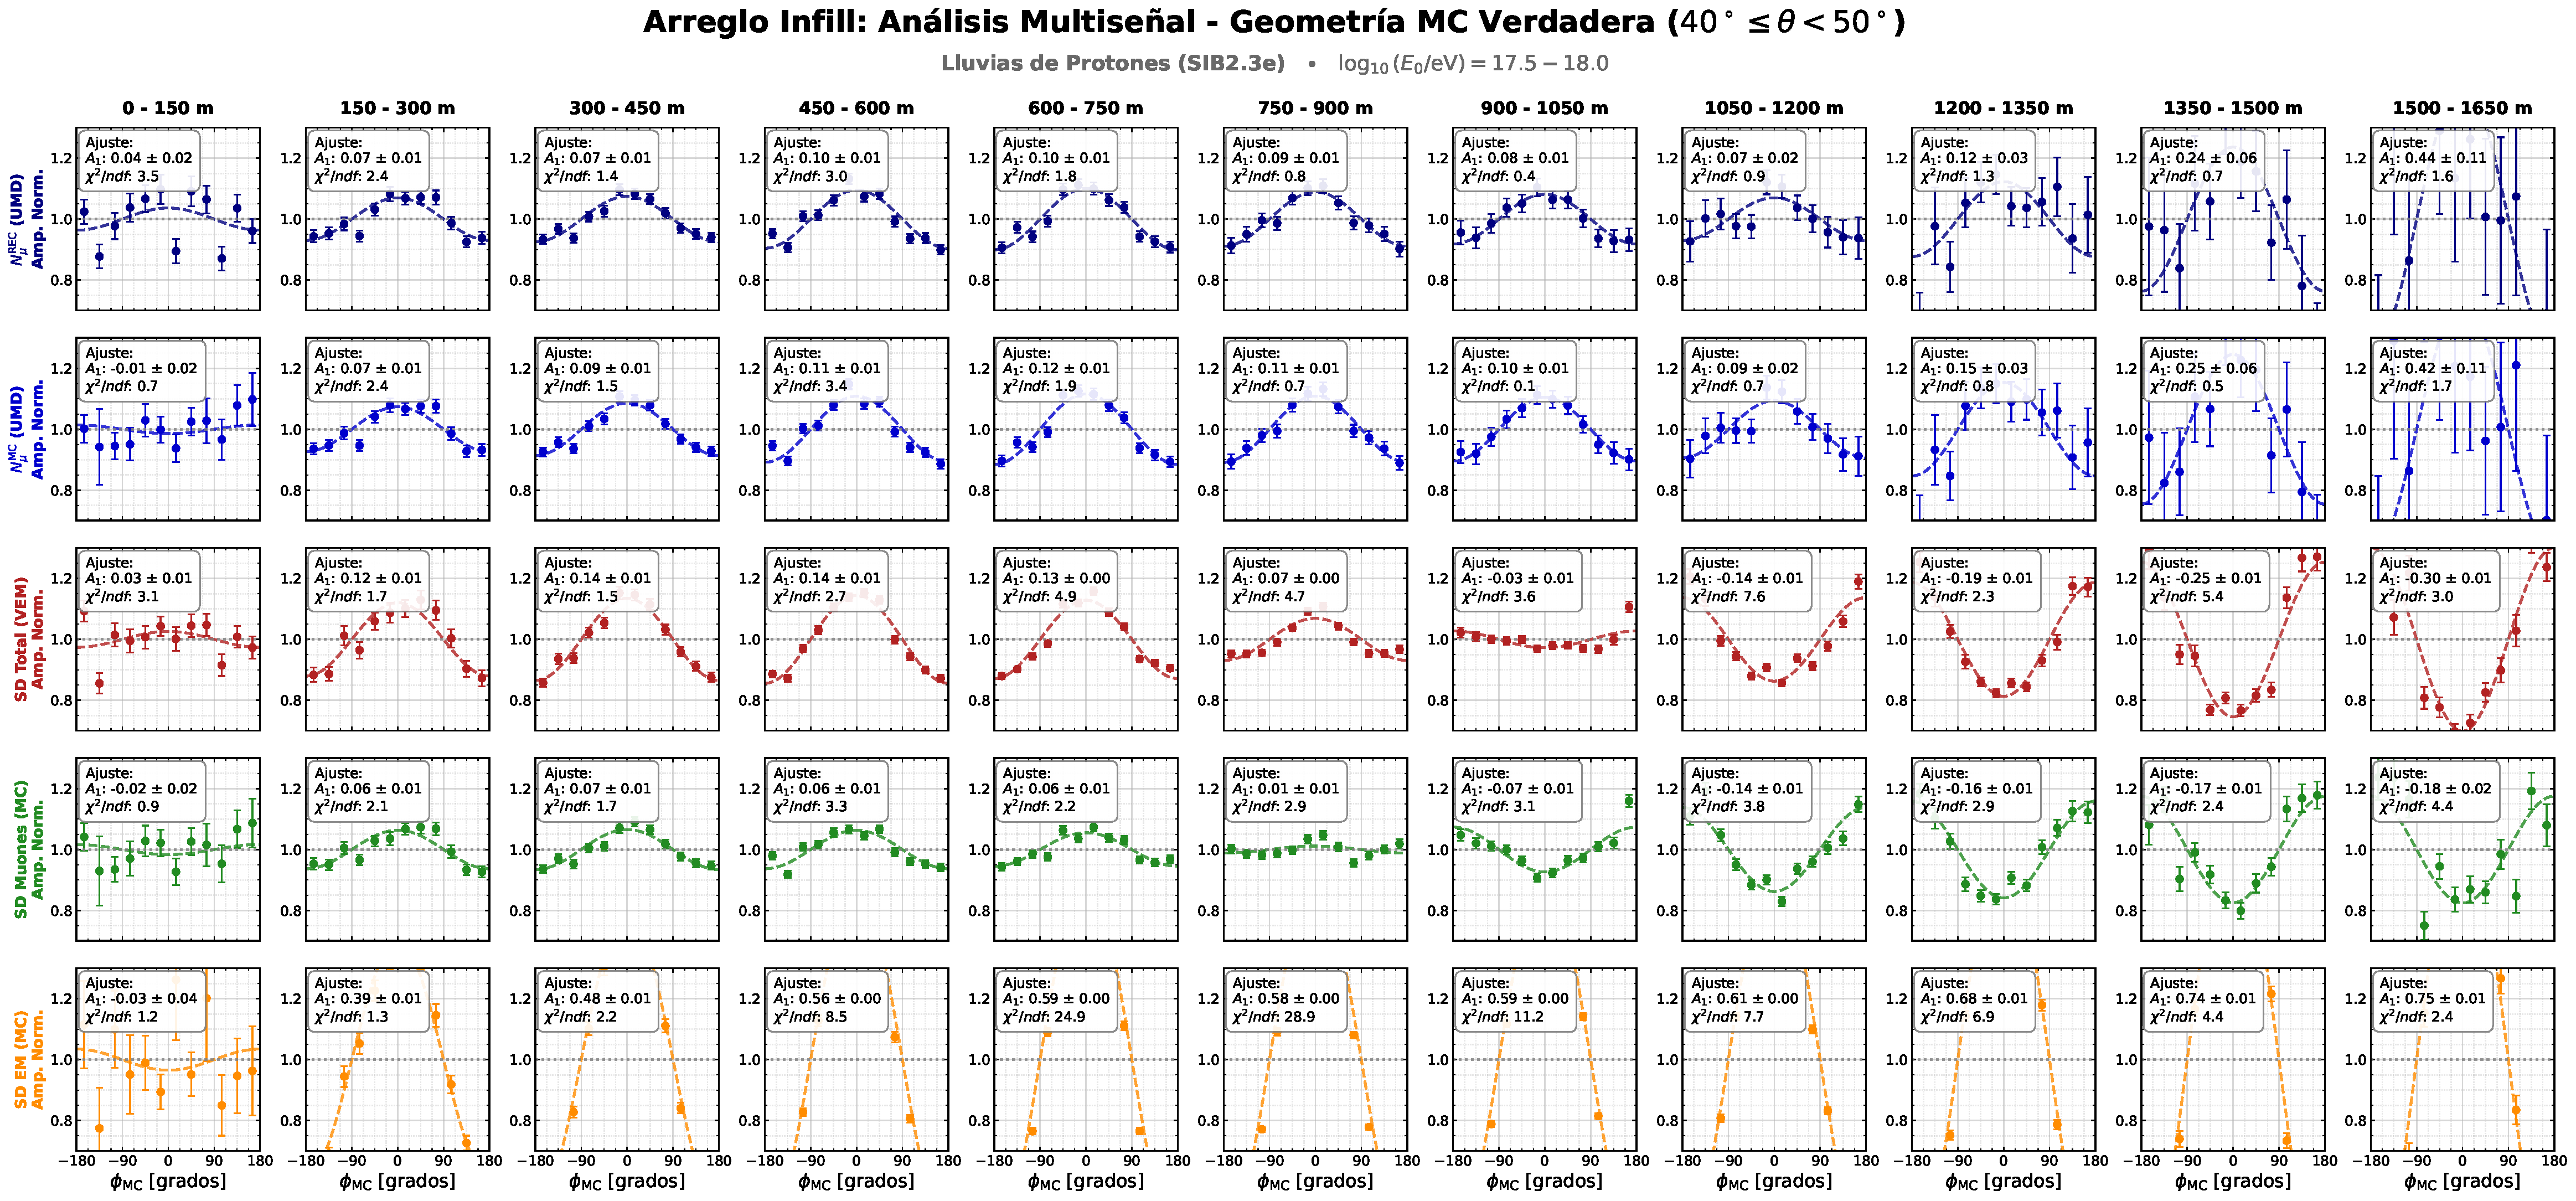
\includegraphics[width=\linewidth]{capitulos/imagenes_capitulos/anexo/Anexo_Grilla_MC_40_50.pdf}
		\caption{Análisis multiseñal de asimetría azimutal forzando la geometría Monte Carlo para lluvias con ángulos cenitales verdaderos entre $40^\circ$ y $50^\circ$.}
		\label{fig:anexo_grilla_mc_40_50}
	\end{figure}
	\clearpage
	
	% --- Bin 50 - 65 ---
	\begin{figure}[H]
		\centering
		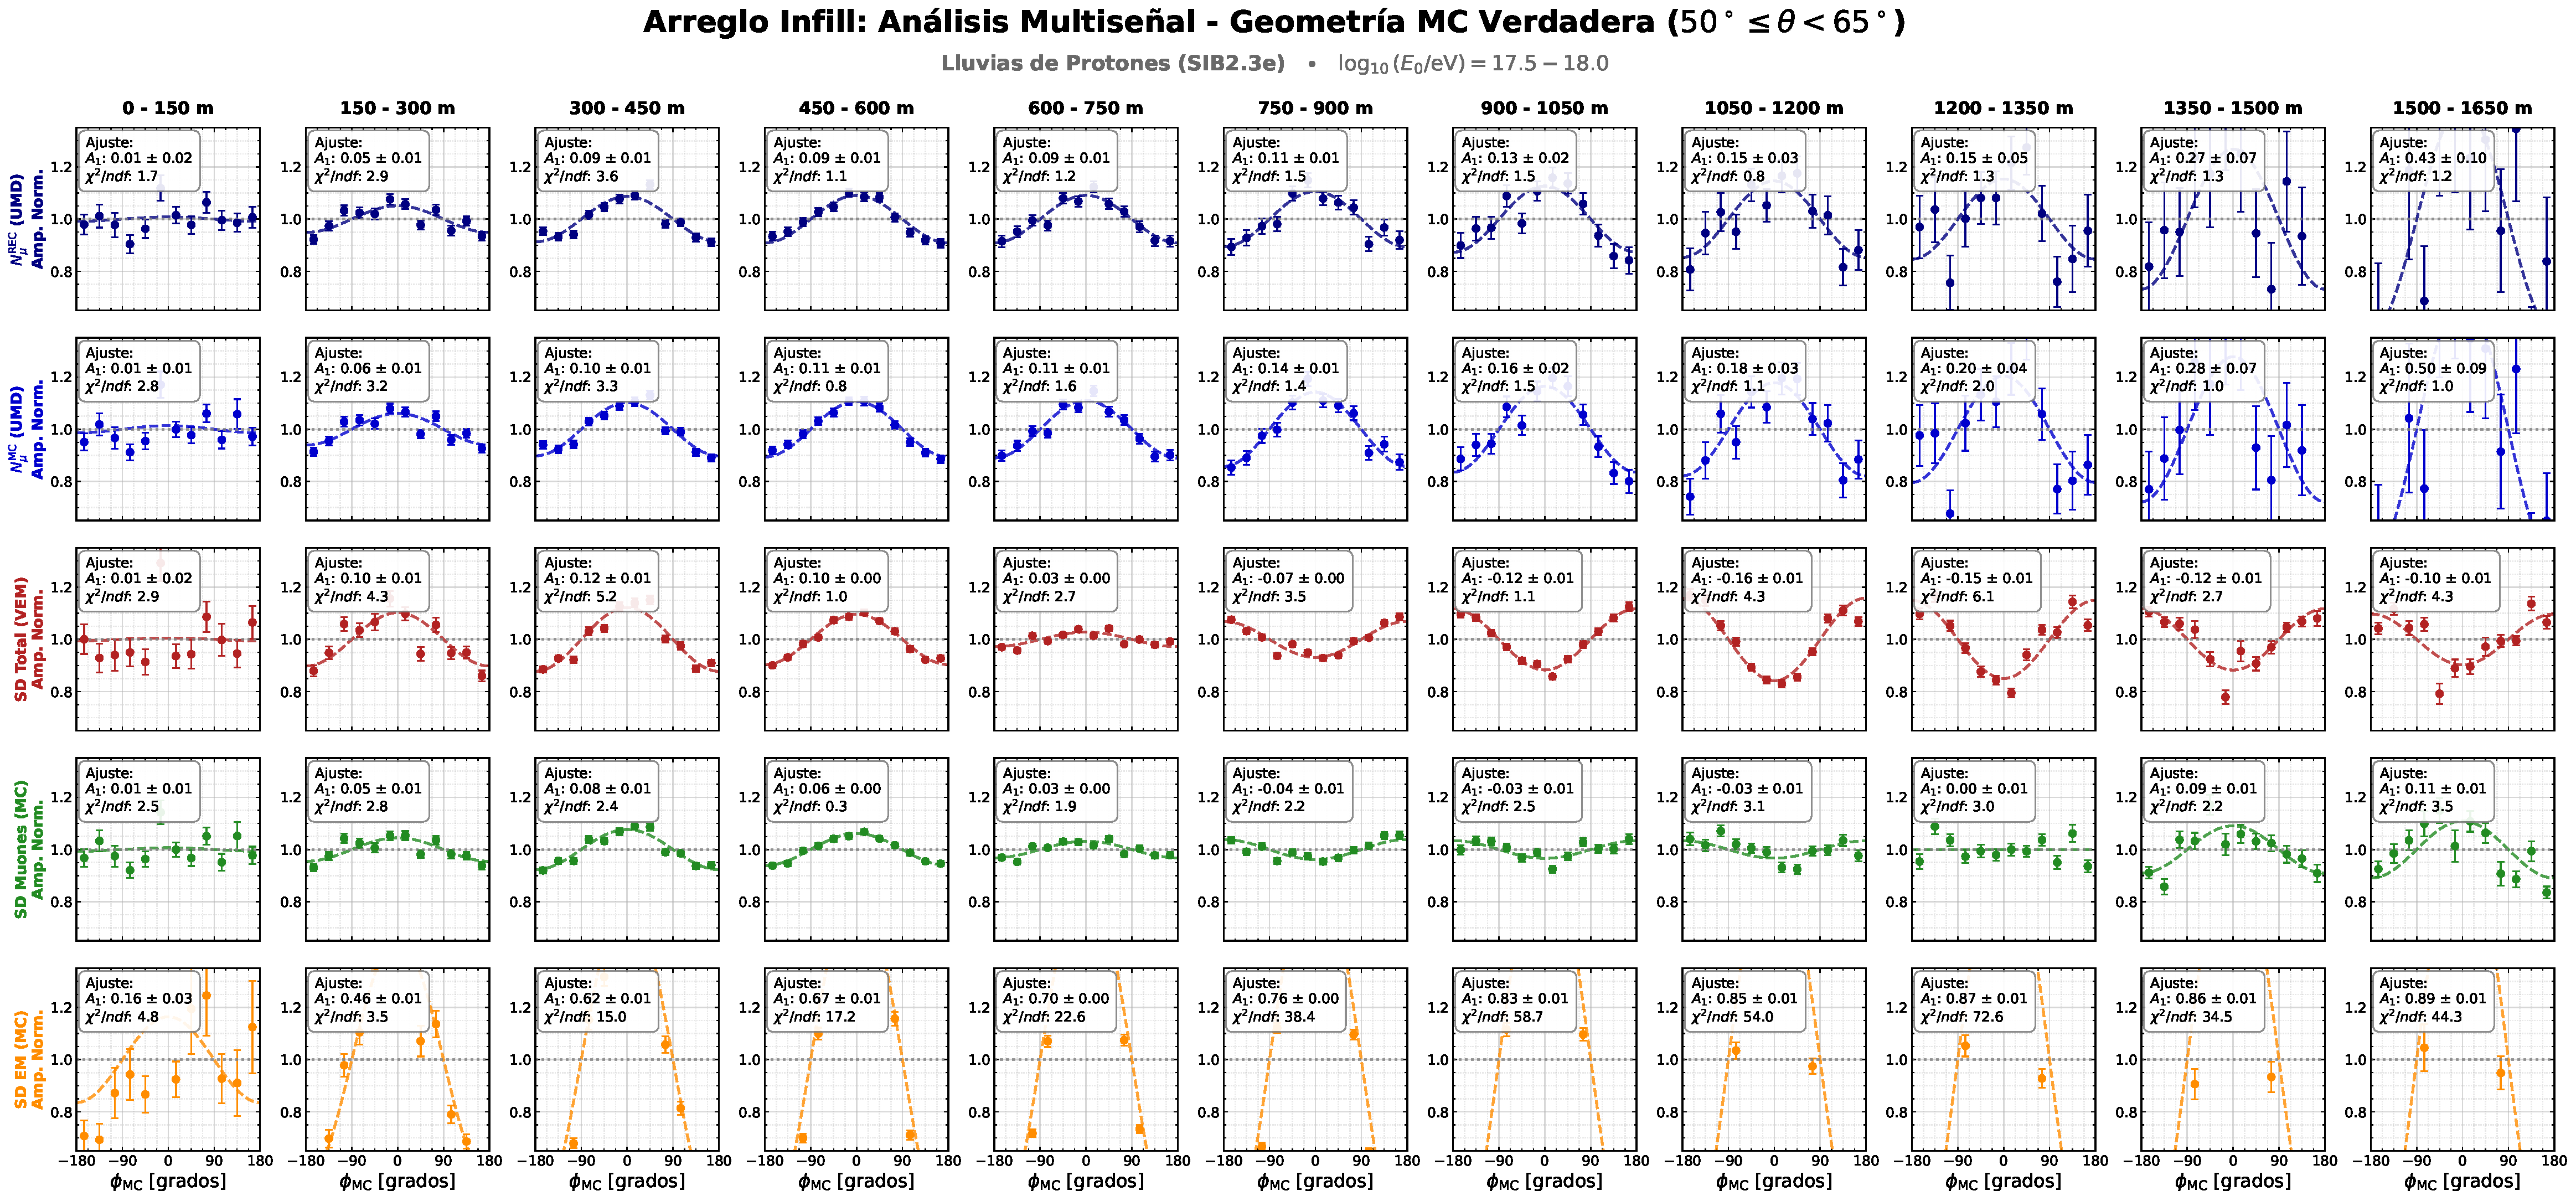
\includegraphics[width=\linewidth]{capitulos/imagenes_capitulos/anexo/Anexo_Grilla_MC_50_65.pdf}
		\caption{Análisis multiseñal de asimetría azimutal forzando la geometría Monte Carlo para lluvias muy inclinadas con ángulos cenitales verdaderos entre $50^\circ$ y $65^\circ$. Se evidencia la persistencia de la modulación asimétrica a grandes distancias del núcleo.}
		\label{fig:anexo_grilla_mc_50_65}
	\end{figure}
	
\end{landscape}


% --- Geometría Reconstruida ---
\newpage % Suele ser buena idea forzar un salto de página entre los distintos modos
\begin{landscape}
	
	% --- Geometría Monte Carlo ---
	\subsection{Geometría Reconstruida}
	\label{anexo:ajustes_infill_rec}
	
	% --- Bin 0 - 10 ---
	\begin{figure}[H]
		\centering
		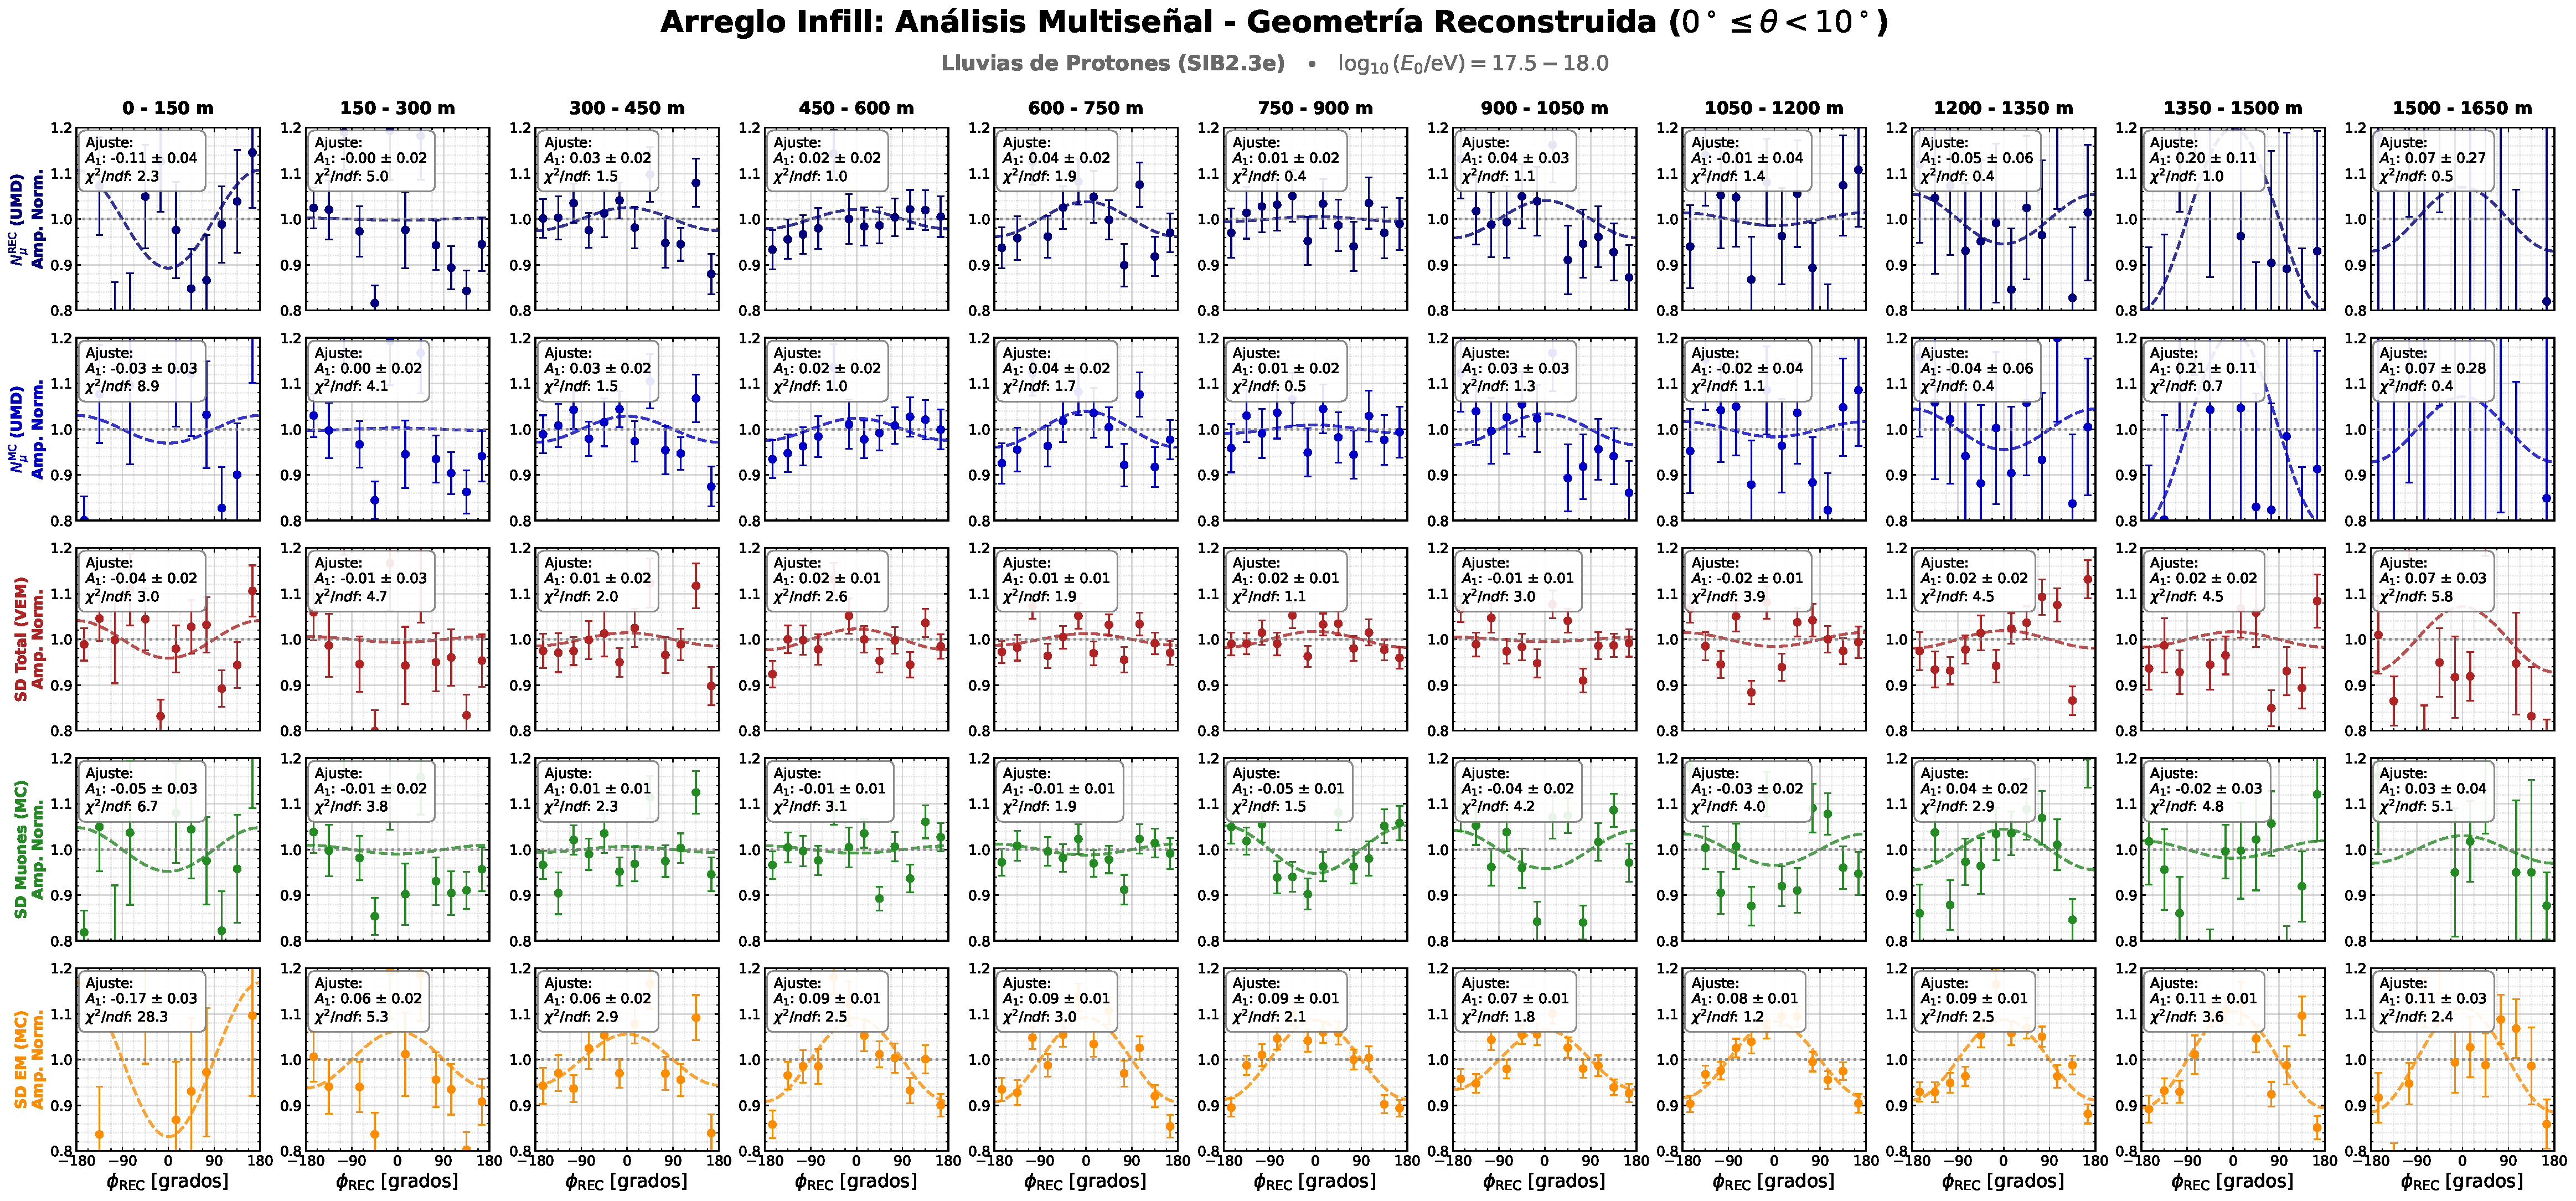
\includegraphics[width=1\linewidth]{capitulos/imagenes_capitulos/anexo/Anexo_Grilla_REC_0_10.pdf}
		\caption{Análisis multiseñal de asimetría azimutal usando la geometría Reconstruida para lluvias con ángulos cenitales verdaderos entre $0^\circ$ y $10^\circ$. Las barras de error representan el error estándar de la media en cada bin angular.}
		\label{fig:anexo_grilla_rec_0_10}
	\end{figure}
	\clearpage
	
	% --- Bin 10 - 20 ---
	\begin{figure}[H]
	\centering
	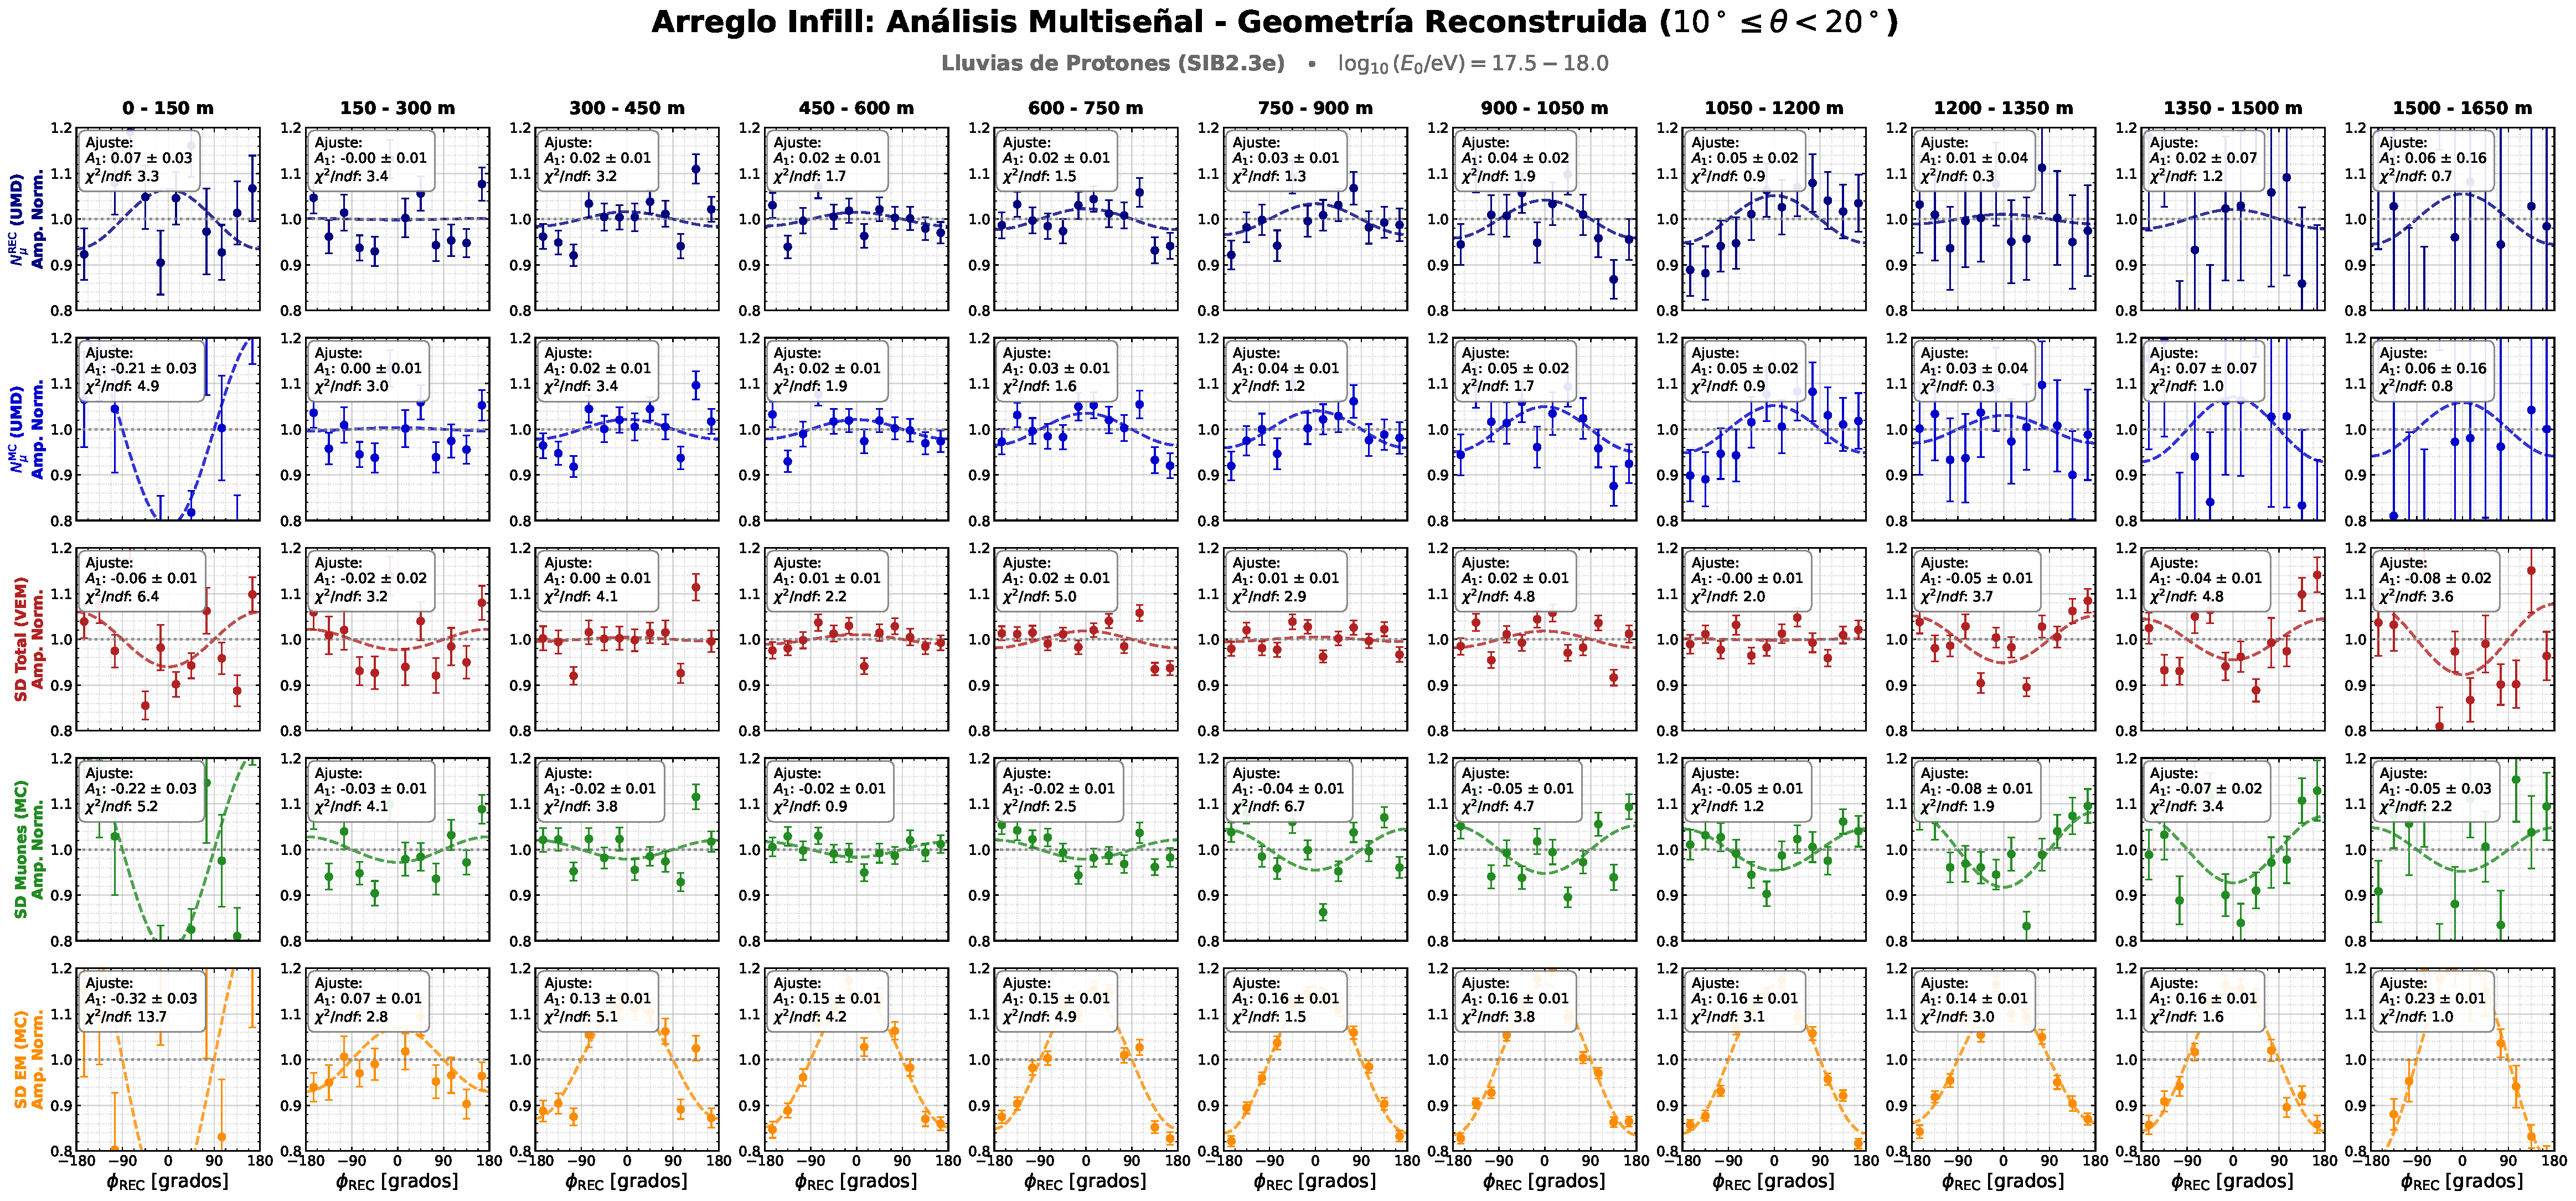
\includegraphics[width=1\linewidth]{capitulos/imagenes_capitulos/anexo/Anexo_Grilla_REC_10_20.pdf}
	\caption{Análisis multiseñal de asimetría azimutal usando la geometría Reconstruida para lluvias con ángulos cenitales verdaderos entre $10^\circ$ y $20^\circ$. Las barras de error representan el error estándar de la media en cada bin angular.}
	\label{fig:anexo_grilla_rec_10_20}
\end{figure}
\clearpage
	
	% --- Bin 20 - 30 ---
	\begin{figure}[H]
	\centering
	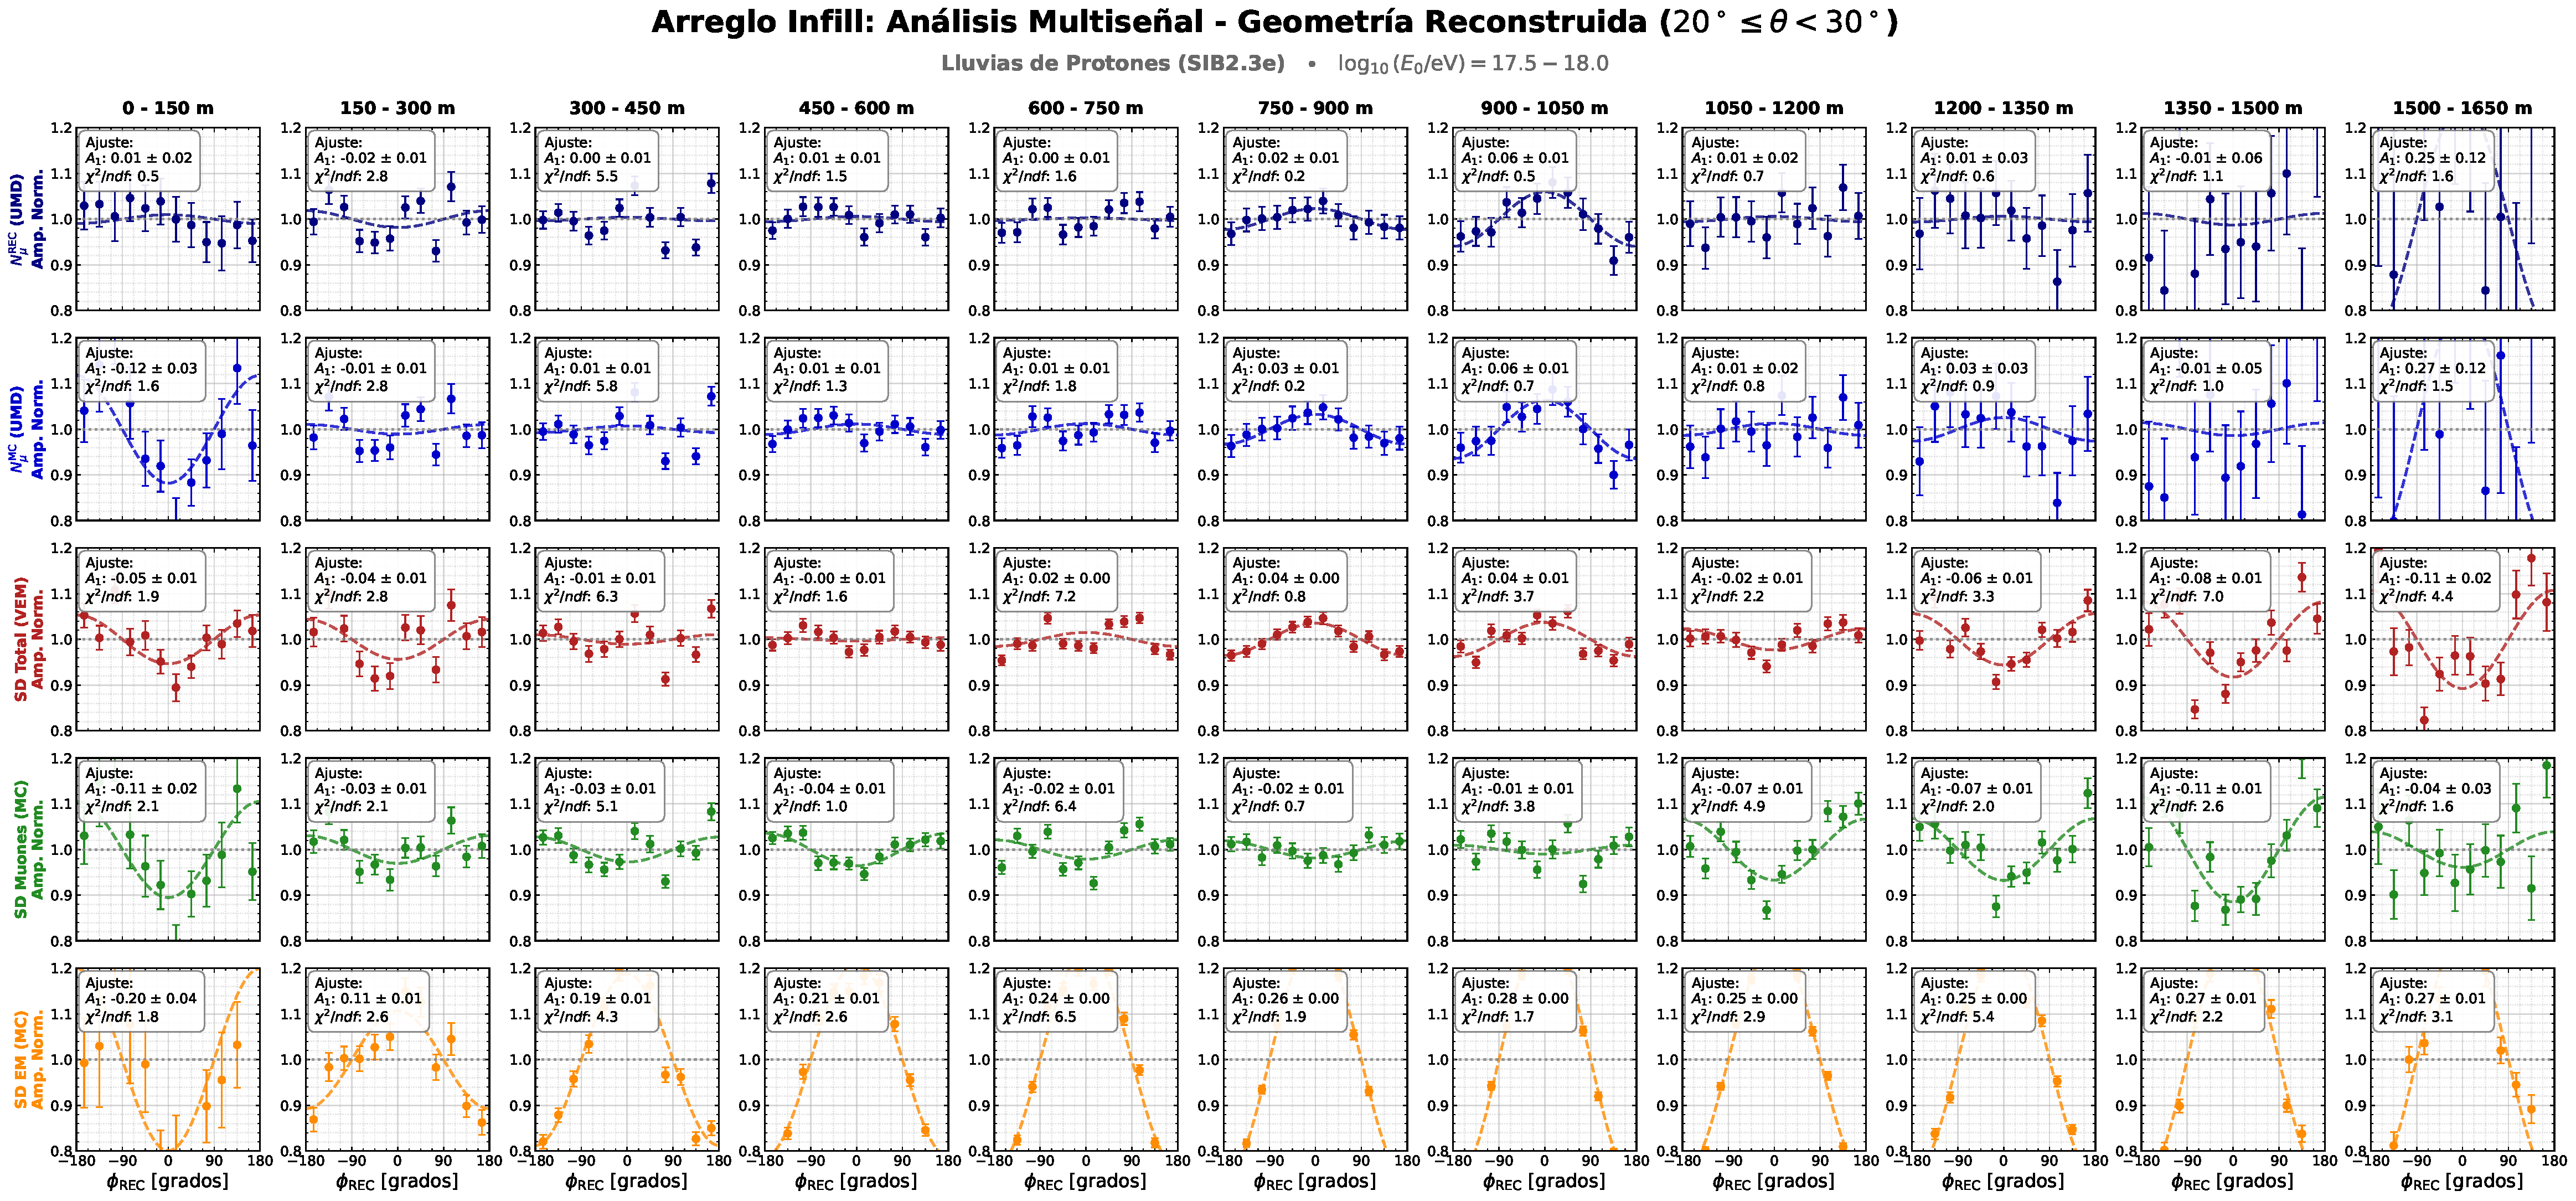
\includegraphics[width=1\linewidth]{capitulos/imagenes_capitulos/anexo/Anexo_Grilla_REC_20_30.pdf}
	\caption{Análisis multiseñal de asimetría azimutal usando la geometría Reconstruida para lluvias con ángulos cenitales verdaderos entre $20^\circ$ y $30^\circ$. Las barras de error representan el error estándar de la media en cada bin angular.}
	\label{fig:anexo_grilla_rec_20_30}
\end{figure}
\clearpage
	
	% --- Bin 30 - 40 ---
	\begin{figure}[H]
	\centering
	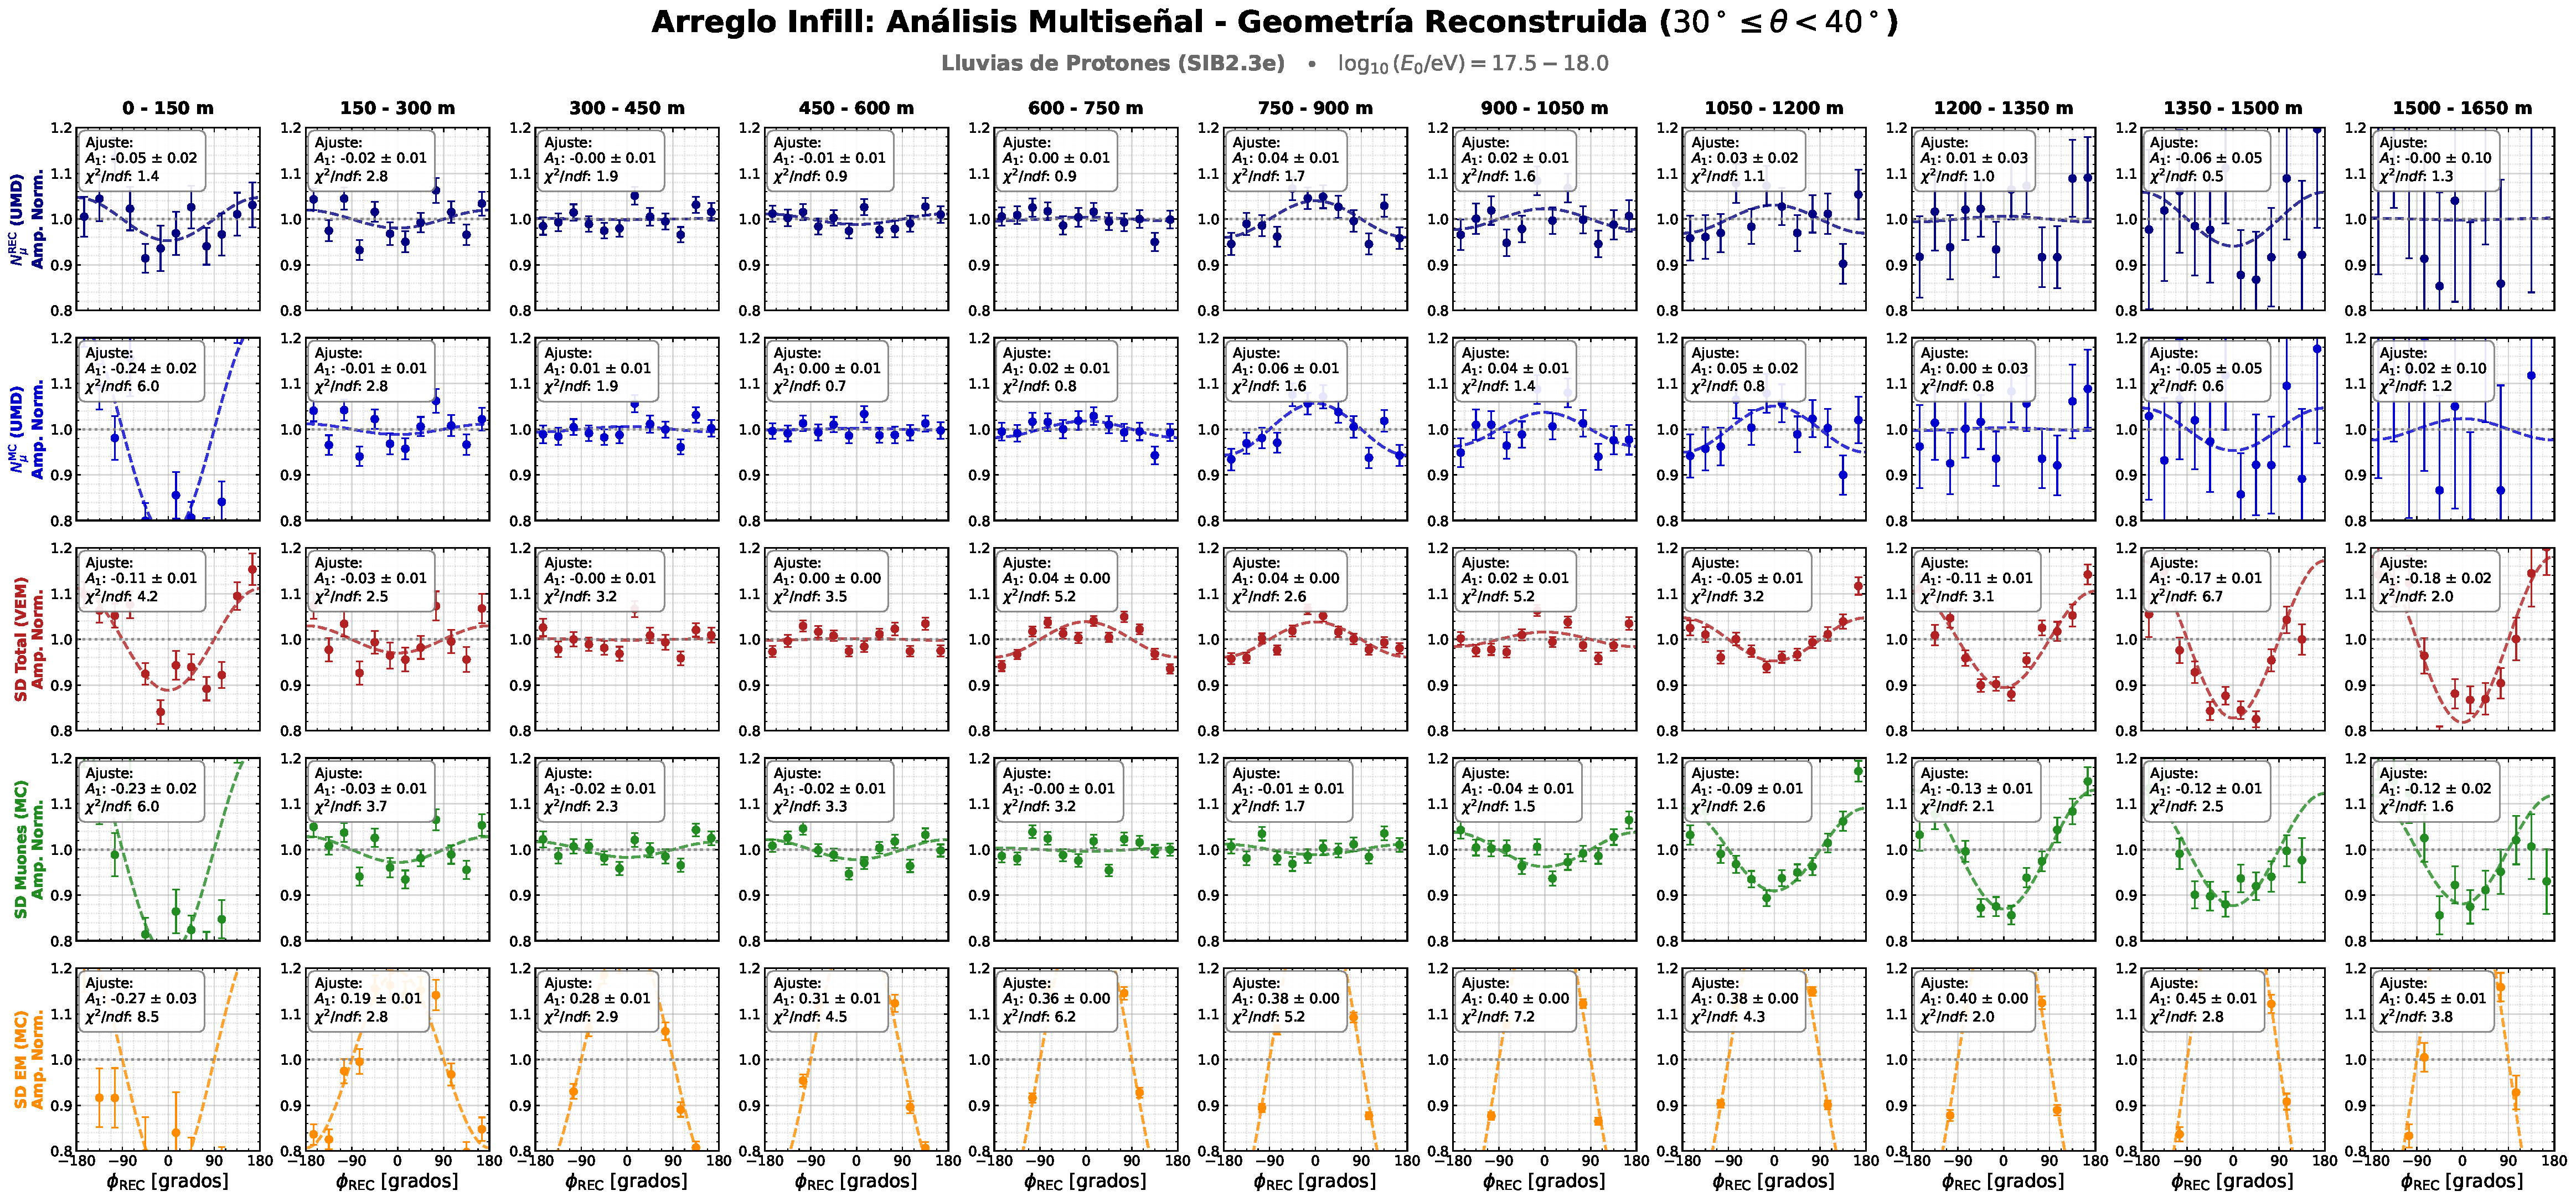
\includegraphics[width=1\linewidth]{capitulos/imagenes_capitulos/anexo/Anexo_Grilla_REC_30_40.pdf}
	\caption{Análisis multiseñal de asimetría azimutal usando la geometría Reconstruida para lluvias con ángulos cenitales verdaderos entre $30^\circ$ y $40^\circ$. Las barras de error representan el error estándar de la media en cada bin angular.}
	\label{fig:anexo_grilla_rec_30_40}
\end{figure}
\clearpage
	
	% --- Bin 40 - 50 ---
	\begin{figure}[H]
	\centering
	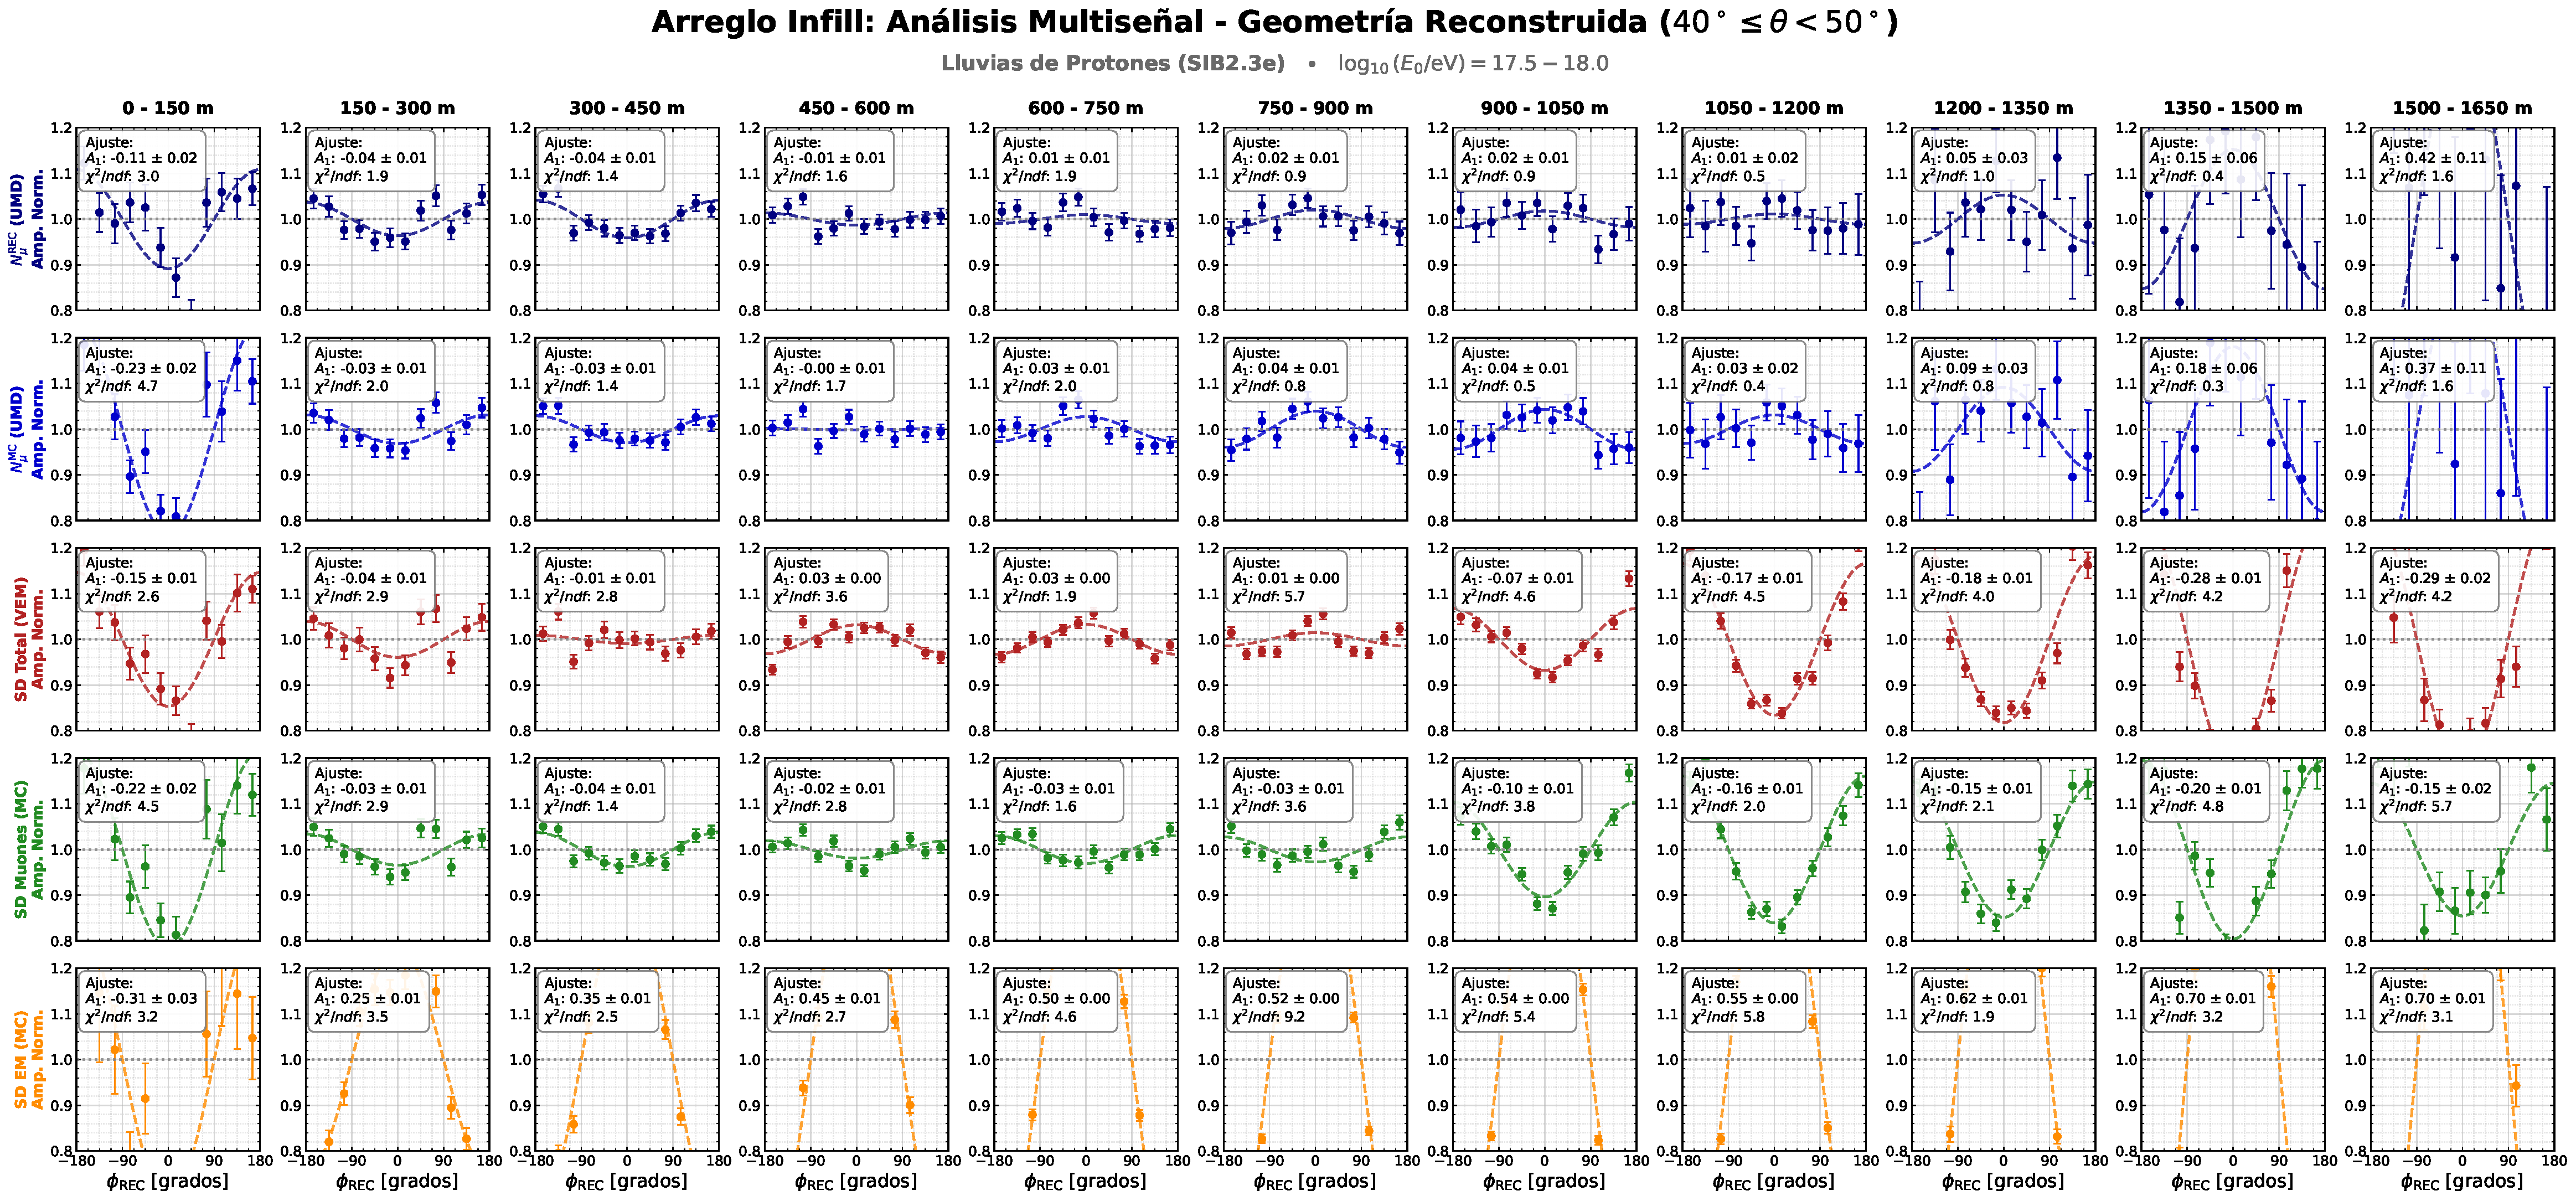
\includegraphics[width=1\linewidth]{capitulos/imagenes_capitulos/anexo/Anexo_Grilla_REC_40_50.pdf}
	\caption{Análisis multiseñal de asimetría azimutal usando la geometría Reconstruida para lluvias con ángulos cenitales verdaderos entre $40^\circ$ y $50^\circ$. Las barras de error representan el error estándar de la media en cada bin angular.}
	\label{fig:anexo_grilla_rec_40_50}
\end{figure}
\clearpage
	
	% --- Bin 50 - 65 ---
	\begin{figure}[H]
	\centering
	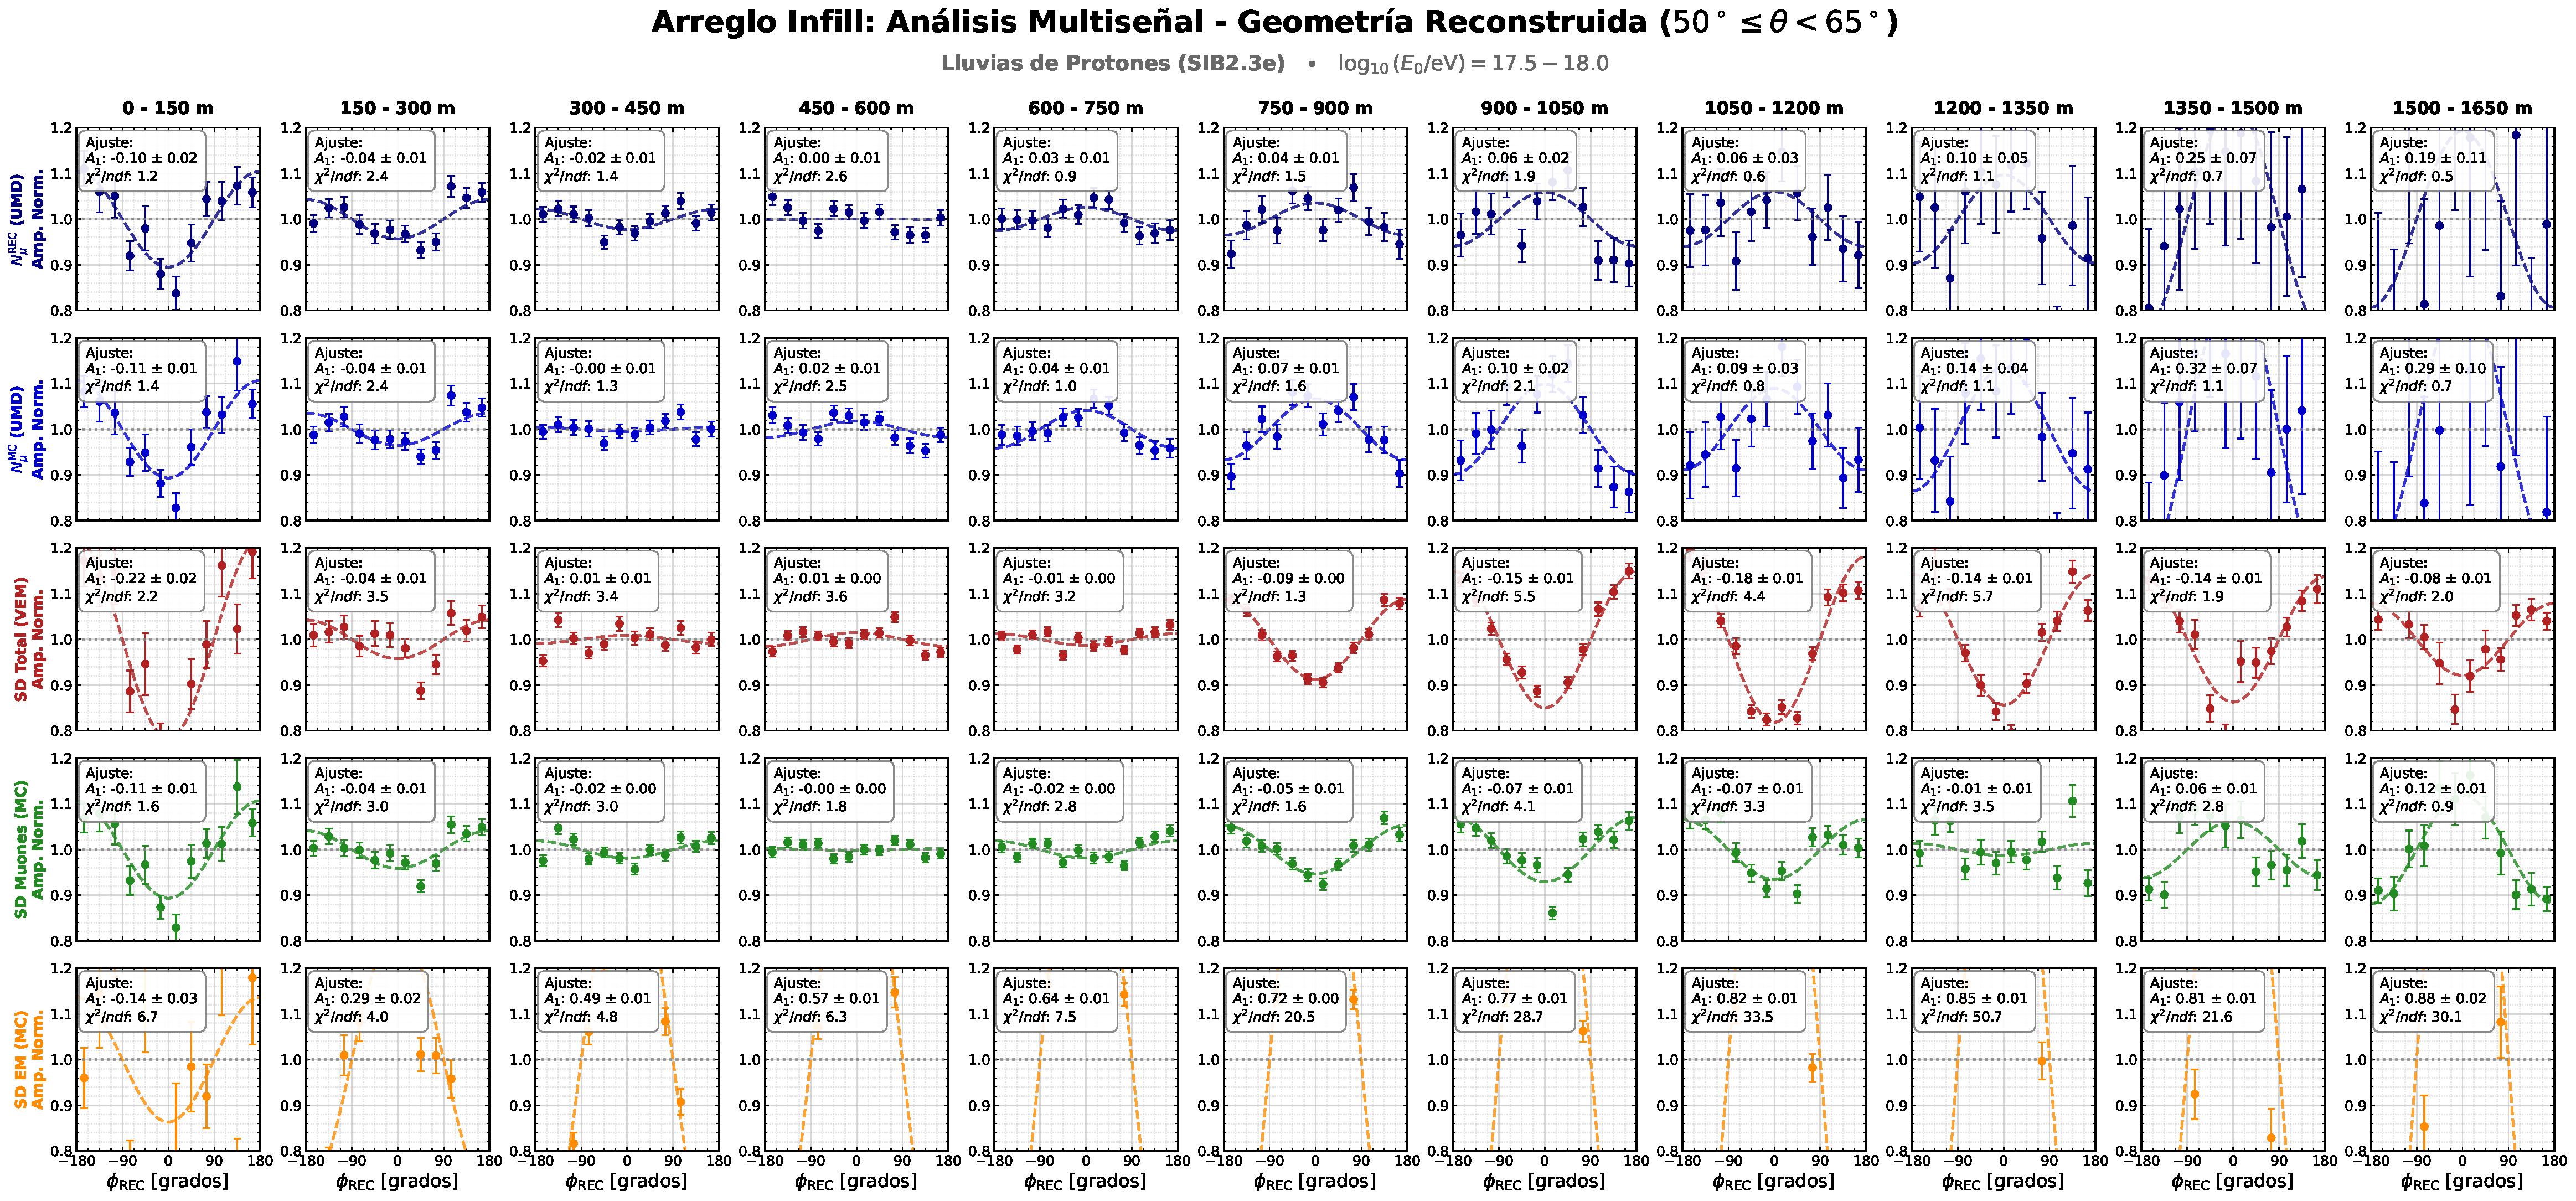
\includegraphics[width=1\linewidth]{capitulos/imagenes_capitulos/anexo/Anexo_Grilla_REC_50_65.pdf}
	\caption{Análisis multiseñal de asimetría azimutal usando la geometría Reconstruida para lluvias con ángulos cenitales verdaderos entre $50^\circ$ y $65^\circ$. Las barras de error representan el error estándar de la media en cada bin angular.}
	\label{fig:anexo_grilla_rec_50_65}
\end{figure}
\clearpage
	
\end{landscape}
% Acá podés ir sumando las figuras para 30-40, 40-50, etc. en modo REC